% $Id: ESMF_usrdoc.tex,v 1.13 2003/05/07 04:34:32 cdeluca Exp 

\documentclass[english]{article}
\usepackage{babel}
\usepackage{supertabular}
\usepackage{html}
\usepackage{times}
\usepackage{graphicx}
\usepackage[T1]{fontenc}

\newcommand{\docmttype}{User's Guide}
\newcommand{\req}[1]{\section{\hspace{.2in}#1}}
\newcommand{\sreq}[1]{\subsection{\hspace{.2in}#1}}
\newcommand{\ssreq}[1]{\subsubsection{\hspace{.2in}#1}}
\newcommand{\mytitle}{\longname \docmttype ~~}
\newcommand{\myversion}{Version 1.0}

\newenvironment
{reqlist}
{\begin{list} {} {} \rm \item[]}
{\end{list}}

%===============================================================================
% User-defined commands
%-------------------------------------------------------------------------------
\newcommand{\longname}{ESMF }
\newcommand{\funcname}{ESMF }
\newcommand{\shortname}{REF}
\newcommand{\myauthors}{ESMF Joint Specification Team:  V. Balaji, Tom Bettge, Byron Boville, Nancy Collins, Tony Craig, Carlos Cruz, Arlindo da Silva, Cecelia DeLuca, Brian Eaton, Bob Hallberg, Chris Hill, Mark Iredell, Rob Jacob, Phil Jones, Brian Kauffman, Jay Larson, John Michalakes, David Neckels, Jim Rosinski, Earl Schwab, Shepard Smithline, Max Suarez, Jon Wolfe, Weiyu Yang, Mike Young, Leonid Zaslavsky}
%===============================================================================
\setlength{\textwidth}{6.5truein}
\setlength{\textheight}{8.5truein}
\setlength{\oddsidemargin}{0in}
\setlength{\unitlength}{1truecm}

\begin{document}

\bodytext{BGCOLOR=white LINK=#083194 VLINK=#21004A}

% Title page

% $Id$
%
% Earth System Modeling Framework
% Copyright 2002-2015, University Corporation for Atmospheric Research, 
% Massachusetts Institute of Technology, Geophysical Fluid Dynamics 
% Laboratory, University of Michigan, National Centers for Environmental 
% Prediction, Los Alamos National Laboratory, Argonne National Laboratory, 
% NASA Goddard Space Flight Center.
% Licensed under the University of Illinois-NCSA License.


\begin{titlepage}

\begin{center}
{\Large Earth System Modeling Framework } \\
\vspace{.25in}
{\Large {\bf \mytitle}} \\
\vspace{.25in}
{\large {\bf \myversion}} \\
\vspace{.5in}
{\large {\it \myauthors}} \\
\vspace{.25in}
{\large {\today}}
\vspace{.25in}
\end{center}

\begin{latexonly}
\vspace{4.5in}
\begin{tabular}{p{5in}p{.9in}}
\hrulefill \\
\noindent http://www.esmf.ucar.edu \\
\end{tabular}
\end{latexonly}

\end{titlepage}
















\newpage
\tableofcontents

\newpage

%\section{Introduction}

\section{Release Notes}

ESMF v2.0 is a first usable release of the Earth System 
Modeling Framework.  While the ESMF still has much growing to do
over the coming years, we expect modelers to find in this release 
tools that benefit real codes.  You may choose to start with the
highest level of functionality in the framework, the software
for representing models as components and coupling them to other
models; or the lowest level, the toolkits for data communication,
I/O, logging, or calendar management.  Wherever you begin, we hope
that you find the ESMF useful, and look forward to hearing your
comments on any aspect of the software.  
Section \ref{sec:Support} 
of this document includes instructions on submitting comments on 
ESMF to our development team.

\section{What is the Earth System Modeling Framework?}

The Earth System Modeling Framework (ESMF) is a structured collection of 
software building blocks that can be used or customized to develop 
Earth system model components, and assemble them into applications.  
The simplest view of the ESMF is that it consists of an {\it infrastructure} 
of utilities and data structures for creating 
model components, and a {\it superstructure} for coupling them.  
User code sits between these two layers, making calls to the infrastructure
libraries beneath it and being scheduled and synchronized by the 
superstructure above it.  The configuration resembles a sandwich, as
shown in Figure~\ref{fig:TheESMFwich}.

The ESMF architecture is scalable, flexible paradigm for building highly 
complex climate, weather, and related applications from components such
as atmospheric models, land models, and data assimilation systems.  The 
ESMF is not a single master application into which all components must fit; 
rather it is a way of developing components so that they can be used 
in many different user-written applications.  Model components that adopt 
ESMF are usable in different contexts without code modification, and may be
incorporated into other ESMF-based modeling systems within the Earth 
science community.  In addition to high-level organization, ESMF provides 
a set of robust, portable, performance optimized libraries for regridding, 
data transfers, I/O, time management, and other common modeling functions.  
ESMF users may choose to extensively rewrite their codes to take advantage 
of the ESMF infrastructure, or they may decide to simply wrap user-written 
components in ESMF interfaces in order to adopt the ESMF architecture and 
utilize framework coupling services.

\section{The ESMF User's Guide}

This {\it ESMF User's Guide} will eventually serve as an introduction for the 
new ESMF user and as a reference for the experienced user.
This edition of the {\it User's Guide} 
is designed to guide you through the introduction process
to the software.  We strongly encourage you
to download the ESMF software and try running a demonstration program, 
{\tt ESMF\_COUPLED\_FLOW}, that illustrates both ESMF utilities and coupling
services.

The next two sections, \ref{sec:Support} and \ref{sec:Submission}, concern 
user support and how to submit comments on the ESMF system to our develoment 
team.  Section \ref{sec:QuickStart} contains a {\it Quick Start} guide that 
explains how to install the ESMF software and 
run the demonstration program.  Section \ref{sec:ArchOver} is an 
architectural overview that describes the framework's basic goals and features.The next few Sections, beginning with \ref{sec:demo}, describe in detail
the {\tt ESMF\_COUPLED\_FLOW} demo application.    
More detail on ESMF structure and operation, such as a description of the 
directory structure and how to run the ESMF self-tests, is provided in Section 
\ref{sec:TechOver}.  Section \ref{sec:Adoption} details the steps 
required to adapt a component for use with ESMF.  Finally, to help you become 
familiar with ESMF terminology, the last section in the {\it User's Guide} is 
a glossary.  

\begin{center}
\begin{figure}
\caption{Schematic of ESMF ``sandwich'' architecture. In this design the framework consists of two parts. An upper level
{\bf Superstructure} layer and a lower-level {\bf Infrastructure} layer. User code is sandwiched between these two layers.}
\label{fig:TheESMFwich}
\scalebox{1.0}{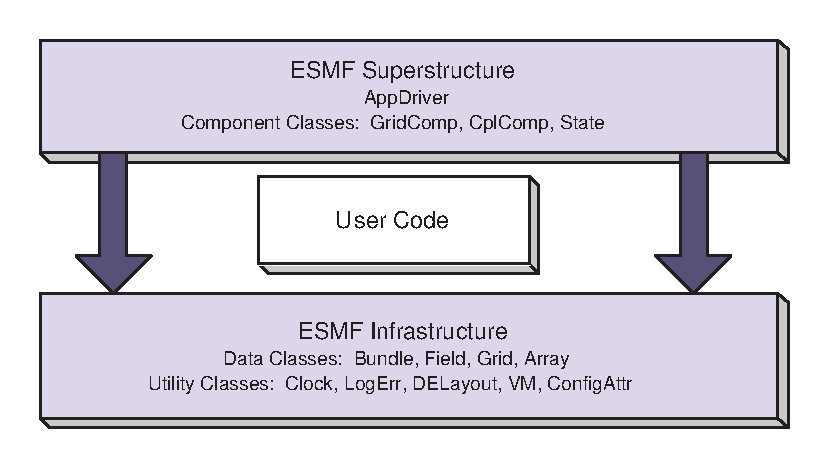
\includegraphics{ESMF_sandwich.eps}}
\end{figure}
\end{center}


















%\section{ESMF Support and Contacts}
\section{How to Contact User Support and Find Additional Information}
\label{sec:Support}
The ESMF team can provide assistance in using the framework in your
applications.
For user support, please contact 
\htmladdnormallink{esmf\_support@ucar.edu}{mailto:esmf_support@ucar.edu}.  

More information on the ESMF project as a whole is available on the 
ESMF website, \htmladdnormallink{http://www.esmf.ucar.edu}{http://www.esmf.ucar.edu}.  
The website includes release notes and known bugs for each version of the
framework, supported platforms, project history, values, and metrics, related projects,
the ESMF management structure, and much more.  Those curious about specific 
interfaces should refer to the \htmladdnormallink
{{\it ESMF Reference Manual for Fortran}}{http://www.esmf.ucar.edu/esmf_releases/public/last/ESMF_refdoc}, which contains a detailed listing and description of 
the ESMF API (this version of the document corresponds to the last public version of the framework).  Also available on the ESMF website is the
\htmladdnormallink{{\it ESMF Developer's Guide}}{http://www.esmf.ucar.edu/documents/dev_guide} 
that details our project procedures and conventions.

\section{How to Submit Comments, Bug Reports, and Feature Requests}
\label{sec:Submission}
We welcome input on any aspect of the ESMF project.  General
questions and comments should be sent to \htmladdnormallink{esmf\_support@ucar.edu}
{mailto:esmf_support@ucar.edu}.




\newpage
%\section{Quick Start}
\section{Quick Start}
\label{sec:QuickStart}

This section gives a brief
description of to how to get the ESMF software, build it, 
and run the self-tests to verify the installation was successful.
More detailed information on each of these steps, as well as
information on running a demonstration application and linking
the ESMF with your own code is found in Sections \ref{sec:TechOver} 
and \ref{sec:TechOver2}.  

\subsection{Downloading ESMF}
\subsubsection{From the ESMF web site}
\label{sec:download}
ESMF is distributed as a source code tar file.  The tar file for the latest
public release, release notes, 
known bugs, supported platforms, documentation, and other related information 
can be found on the ESMF website, under the {\bf Download} tab:
\begin{verbatim}
    http://www.esmf.ucar.edu -> Download
\end{verbatim}
The source code for all other releases including the HEAD of the CVS trunk and the
last stable version can be found by following the {\bf View All Releases} link on the left hand navigation bar under {\bf Download}:
\begin{verbatim}
    http://www.esmf.ucar.edu -> Download -> View All Releases
\end{verbatim}

\subsubsection{From the SourceForge website}
ESMF can also be downloaded from the SourceForge website
from the {\bf Files} link on that website.
\begin{verbatim}
    http://sourceforge.net/projects/esmf -> Files
\end{verbatim}
Follow the directions on that web page to download a tar file.  

\subsection{Unpacking the download}
The source code comes as a zipped tar file. First unzip the file:
\begin{verbatim}
gunzip esmf*.tar.gz
\end{verbatim}

Then untar the file:
\begin{verbatim}
tar -xf esmf*.tar
\end{verbatim}

This will create a directory called {\tt esmf}.

\subsection{Directory Structure}
The current list of directories includes the following:
\begin{itemize}
\item README
\item application
\item build
\item build\_config
\item makefile
\item scripts
\item src
\end{itemize}

The build\_config directory contains subdirectories for
different operating system, compiler combinations. This is
a useful area to examine if porting ESMF to a new platform.

\subsection{Building ESMF}

After downloading and unpacking the ESMF tar file, the build procedure is:
\begin{enumerate}
\item Set the required environment variables. 
\item Type {\tt gmake info} to view and verifty your settings
\item Type {\tt gmake } to build the library.
\item Type {\tt gmake check } to run self-tests to verify
the build was successful.
\end{enumerate}
See the following sections for more information on each of these steps.

\subsubsection{Environment Variables}

The syntax for setting environment variables depends on which shell
you are running.  Examples of the two most common ways to set 
an environment variable are:
\begin{description}
\item[ksh] {\tt  export ESMF\_DIR=/home/joeuser/esmf}
\item[csh] {\tt  setenv ESMF\_DIR /home/joeuser/esmf}
\end{description}

The shell environment variables listed below are the ones most
frequently used.  There are others which address needs on specific
platforms or are needed under more unusual circumstances; 
see Section \ref{sec:TechOver} for the full list.  
\begin{description}

\item[ESMF\_DIR]
The environment variable {\tt ESMF\_DIR} must be set to the full pathname 
of the top level ESMF directory before building the framework.  This is the 
only environment variable which is required to be set on all platforms under 
all conditions.

\item[ESMF\_BOPT]
This environment variable controls the build option. To make a debuggable
version of the library set {\tt ESMF\_BOPT} to {\tt g} before building. The
default is {\tt O} (capital oh) which builds an optimized version of the 
library. If {\tt ESMF\_BOPT} is {\tt O}, {\tt ESMF\_OPTLEVEL} can also be set
to a numeric value between 0 and 4 to select a specific optimization level.

\item[ESMF\_COMM]
On systems with a vendor-supplied MPI communications library the vendor library 
is chosen by default for communications and {\tt ESMF\_COMM} need not be set.
For other systems (e.g. Linux or Darwin) a multitude of MPI implementations is
available and {\tt ESMF\_COMM} must be set to indicate which implementation is
used to build the ESMF library. Set {\tt ESMF\_COMM} according to your situation
to: {\tt mpich, mpich2, lam, openmpi} or {\tt intelmpi}. {\tt ESMF\_COMM} may
also be set to {\tt user} indicating that the user will set all the required
flags using advanced ESMF environment variables.

Alternatively, ESMF comes with a single-processor MPI-bypass library which is
the default for Linux and Darwin systems. To force the use of this bypass
library set {\tt ESMF\_COMM} equal to "mpiuni".

\item[ESMF\_COMPILER]
The ESMF library build requires a working Fortran90 and C++ compiler. On 
platforms that don't come with a single vendor supplied compiler suite
(e.g. Linux or Darwin) {\tt ESMF\_COMPILER} must be set to select which Fortran
and C++ compilers are being used to build the ESMF library. Notice that setting
the {\tt ESMF\_COMPILER} variable does {\em not} affect how the compiler
executables are located on the system. {\tt ESMF\_COMPILER} (together with
{\tt ESMF\_COMM}) affect the name that is expected for the compiler executables.
Furthermore, the {\tt ESMF\_COMPILER} setting is used to select compiler and
linker flags consistent with the compilers indicated.

By default Fortran and C++ compiler executables are expected to be located in
a location contained in the user's {\tt PATH} environment variable. This means
that if you cannot locate the correct compiler executable via the {\tt which}
command on the shell prompt the ESMF build system won't find it either!

There are advanced ESMF environment variables that can be used to select 
specific compiler executables by specifying the full path. This can be used to
pick specific compiler executables without having to modify the {\tt PATH}
environment variable.

Use 'gmake info' to see which compiler executables the ESMF build system will
be using according to your environment variable settings.

To see possible values for {\tt ESMF\_COMPILER}, cd to 
{\tt \$ESMF\_DIR/build\_config} and list the directories there. The first part 
of each directory name corresponds to the output of 'uname -s' for this 
platform. The second part contains possible values for {\tt ESMF\_COMPILER}. In
some cases multiple combinations of Fortran and C++ compilers are possible, e.g.
there is {\tt intel} and {\tt intelgcc} available for Linux. Setting 
{\tt ESMF\_COMPILER} to {\tt intel} indicates that both Intel Fortran and 
C++ compilers are used, whereas {\tt intelgcc} indicates that the Intel Fortran
compiler is used in combination with GCC's C++ compiler.

If you do not find a configuration that matches your situation you will need to
port ESMF.

\item[ESMF\_ABI]
If a system supports 32-bit and 64-bit (pointer wordsize) application binary
interfaces (ABIs), this variable can be set to select which ABI to use. Valid 
values are {\tt 32} or {\tt 64}. By default the most common ABI is chosen.

\item[ESMF\_SITE]
The SourceForge {\tt esmfcontrib} repository contains makefiles which have 
already been customized for certain machines.  If one exists for your site 
and you wish to use it, download the corresponding files into the 
{\tt build\_contrib} directory and set {\tt ESMF\_SITE} to your location
(which corresponds to the last part of the directory name).  See the 
SourceForge site {\tt http://sourceforge.net/projects/esmfcontrib} for more 
information.

\item[ESMF\_INSTALL\_PREFIX]
This variable specifies the prefix of the installation path used during the
installation process accessible thought the install target. Libraries, F90
module files, header files and documentation all are installed relative to
{\tt ESMF\_INSTALL\_PREFIX} by default. The {\tt ESMF\_INSTALL\_PREFIX} may be
provided as absolute path or relative to {\tt ESMF\_DIR}.

\end{description}

\subsubsection{gmake info}
{\tt gmake info} is a command that assists the user in verifying that the ESMF 
variables have been set appropriatly.
It also tells the user the paths to various libararies e.g. MPI that are set on the system.  The user to review this
information to verify their settings. In the case of a build failure, this information is invaluable and will be the
first thing asked for by the ESMF support team. Below is an {/b example output} from {/tt gmake info}:  
\begin{verbatim}
--------------------------------------------------------------
Make version:
GNU Make version 3.79, by Richard Stallman and Roland McGrath.
Built for powerpc-apple-darwin7.0
Copyright (C) 1988, 89, 90, 91, 92, 93, 94, 95, 96, 97, 98, 99
        Free Software Foundation, Inc.
This is free software; see the source for copying conditions.
There is NO warranty; not even for MERCHANTABILITY or FITNESS FOR A
PARTICULAR PURPOSE.

Report bugs to <bug-make@gnu.org>.


--------------------------------------------------------------
Fortran Compiler version:
Pro Fortran 9.0
ERROR: No input files.

--------------------------------------------------------------
C++ Compiler version:
g++ (GCC) 3.3 20030304 (Apple Computer, Inc. build 1666)
Copyright (C) 2002 Free Software Foundation, Inc.
This is free software; see the source for copying conditions.  There is NO
warranty; not even for MERCHANTABILITY or FITNESS FOR A PARTICULAR PURPOSE.


--------------------------------------------------------------
ESMF_VERSION_STRING ``3.0.1''
--------------------------------------------------------------

--------------------------------------------------------------
 * ESMF environment variables *
ESMF_DIR: /Users/murphys/esmf_head
ESMF_OS:                Darwin
ESMF_MACHINE:           default
ESMF_ABI:               32
ESMF_COMPILER:          absoft
ESMF_BOPT:              O
ESMF_COMM:              mpiuni
ESMF_SITE:              default
ESMF_EXHAUSTIVE:        OFF
ESMF_PTHREADS:          ON
ESMF_TESTWITHTHREADS:   OFF
ESMF_ARRAY_LITE:        FALSE
ESMF_NO_INTEGER_1_BYTE: FALSE
ESMF_NO_INTEGER_2_BYTE: FALSE
ESMF_FORTRANSYMBOLS:    default

--------------------------------------------------------------
 * ESMF environment variables pointing to 3rd party software *
--------------------------------------------------------------
 * ESMF environment variables for final installation *
ESMF_INSTALL_PREFIX:    ./DEFAULTINSTALLDIR
ESMF_INSTALL_HEADERDIR: include
ESMF_INSTALL_MODDIR:    mod/modO/Darwin.absoft.32.mpiuni.default
ESMF_INSTALL_LIBDIR:    lib/libO/Darwin.absoft.32.mpiuni.default
ESMF_INSTALL_DOCDIR:    doc


--------------------------------------------------------------
 * Compilers, Linkers, Flags, and Libraries *
Location of the preprocessor:      /usr/bin/gcc
Location of the Fortran compiler:  /Applications/Absoft/bin/f90
Location of the Fortran linker:    /Applications/Absoft/bin/f90
Location of the C++ compiler:      /usr/bin/g++
Location of the C++ linker:        /usr/bin/g++
--------------------------------------------------------------
 * ESMF environment variables for final installation *
ESMF_INSTALL_PREFIX:    ./DEFAULTINSTALLDIR
ESMF_INSTALL_HEADERDIR: include
ESMF_INSTALL_MODDIR:    mod/modO/Darwin.absoft.32.mpiuni.default
ESMF_INSTALL_LIBDIR:    lib/libO/Darwin.absoft.32.mpiuni.default
ESMF_INSTALL_DOCDIR:    doc


--------------------------------------------------------------
 * Compilers, Linkers, Flags, and Libraries *
Location of the preprocessor:      /usr/bin/gcc
Location of the Fortran compiler:  /Applications/Absoft/bin/f90
Location of the Fortran linker:    /Applications/Absoft/bin/f90
Location of the C++ compiler:      /usr/bin/g++
Location of the C++ linker:        /usr/bin/g++

Fortran compiler flags:
ESMF_F90COMPILEOPTS: -O -YEXT_NAMES=LCS -YEXT_SFX=_
ESMF_F90COMPILEPATHS: -p/Users/murphys/esmf_head/mod/modO/Darwin.absoft.32.mpiuni.default -I/Users/murphys/esmf_head/src/inc\
lude
ESMF_F90COMPILECPPFLAGS:  -DS32=1 -DESMF_MPIUNI

Fortran linker flags:
ESMF_F90LINKOPTS:
ESMF_F90LINKPATHS: -L/Users/murphys/esmf_head/lib/libO/Darwin.absoft.32.mpiuni.default
ESMF_F90LINKRPATHS:
ESMF_F90LINKLIBS:  -lstdc++
ESMF_F90ESMFLINKLIBS: -lesmf  -lstdc++
C++ compiler flags:
ESMF_CXXCOMPILEOPTS: -O
ESMF_CXXCOMPILEPATHS: -I/Users/murphys/esmf_head/src/include -I/Users/murphys/esmf_head/src/Infrastructure/stubs/mpiuni
ESMF_CXXCOMPILECPPFLAGS: -DS32=1 -D__SDIR__='src/doc' -DESMF_MPIUNI

C++ linker flags:
ESMF_CXXLINKOPTS:
ESMF_CXXLINKPATHS: -L/Users/murphys/esmf_head/lib/libO/Darwin.absoft.32.mpiuni.default -L/Applications/Absoft/lib
ESMF_CXXLINKRPATHS:
ESMF_CXXLINKLIBS:  -lf90math -lfio -lac -lf77math -lm
ESMF_CXXESMFLINKLIBS: -lesmf  -lf90math -lfio -lac -lf77math -lm


--------------------------------------------------------------
Compiling on Mon May 14 14:54:47 MDT 2007 on glass.scd.ucar.edu
Machine characteristics: Darwin glass.scd.ucar.edu 7.9.0 Darwin Kernel Version 7.9.0: Wed Mar 30 20:11:17 PST 2005; root:xnu\
/xnu-517.12.7.obj~1/RELEASE_PPC Power Macintosh powerpc
==============================================================
\end{verbatim}


\subsubsection{GNU make}
The ESMF build system uses the GNU make program; it is normally named 
{\tt gmake} but may also be simply {\tt make} or {\tt gnumake} on some 
platforms.  ESMF does not use configure or autoconf;  the selection of 
various options is done by
setting environment variables before building the framework. 

\subsubsection{Building Makefile Targets}

The makefiles follow the GNU target standards where possible.
The most frequently used targets for building are listed below:
\begin{description}
\item[lib] build the ESMF libraries only (default)
\item[all] build the libraries, unit and system tests, examples, and demos
\item[doc] build the documentation (requires specific latex macros packages
and additional utilities; see Section \ref{sec:TechOver} for more details
on the requirements).  
\item[info] print out extensive system configuration information about what
           compilers, libraries, paths, flags, etc are being used
\item[clean] remove all files built for this platform/compiler/wordsize.
\item[clobber] remove all files built for all architectures
\item[install] install the ESMF library in a custom location
\end{description}


\subsubsection{Testing Makefile Targets}

To build and run the unit and system tests in non-exhaustive mode, type:
\begin{verbatim}
gmake check
\end{verbatim}
A summary report of success and failures will be printed out at the end.

\noindent Other test-related targets are:
\begin{description}
\item[all\_tests] build and run all available tests and demos
\item[build\_all\_tests] build tests only, do not execute
\item[run\_all\_tests] run tests without rebuilding and print a
summary of the results
\item[check\_all\_tests] 
print out the results summary without re-executing the tests again
\item[clean\_all\_tests] remove all test and demo executables 
\end{description}

For all the targets listed above, the string {\tt all\_tests} can be
replaced with one of the strings listed below to select a
specific type of test:
\begin{description}
\item[unit\_tests] unit tests exercise a single part of the system
\item[system\_tests] system tests combine functions across the system
\item[examples] examples contain code illustrating a single type of function
\item[demos] demos are example applications showing the use of the system
\end{description}
For example, {\tt gmake build\_examples} recompiles the example programs but 
does not execute them.  {\tt gmake clean\_system\_tests} removes all
executables and files associated with the system tests.

For the unit tests only, there is an additional environment variable
which affects how the tests are built:
\begin{description}
\item[ESMF\_EXHAUSTIVE]
If this variable is set to {\tt ON} before compiling the unit tests,
longer and more exhaustive unit tests will be run.  Note that this is a
compile-time and not run-time option.
\end{description}



%\section{ESMF Architectural Overview}
% $Id: ESMF_archoverview.tex,v 1.3 2003/05/07 18:31:31 cdeluca Exp $

\section{Architectural Overview}
\label{sec:ArchOver}
The ESMF architecture is characterized by the layering strategy shown in figure \ref{fig:TheESMFwich}. In this architectural pattern user code components that implement the {\it science} elements of an algorithm, for example evaluating
finite-difference calculations or radiation physics terms, are sandwiched between two layers. The upper layer is
denoted the {\bf Superstructure} layer and the lower layer the {\bf Infrastructure} layer. The role of the {\bf Superstructure}
layer is to provide a shell which encompasses user code and provides a context for interconnecting input and output
data streams between components. The key elements of the {\bf Superstructure} layer are described in section \ref{sec:superstructure}.
These elements include the extensible classes that represent envelope user code components, ensuring that all
components present consistent interfaces. The {\bf Infrastructure} layer provides a foundation that developers of
user components can use to speed construction and to ensure consistent, guaranteed behavior of components.
The elements of the {\bf Infrastructure} layer include constructs to support parallel processing with data types tailored
to Earth science applications, specialized libraries to support consistent time and calendar management and
performance, error handling and scalable I/O tools. The {\bf Infrastructure} layer is described in section \ref{sec:infrastructure}.
A hierarchical combination of {\bf Superstructure}, user code components and Infrastructure are joined together
to form what is termed an {\it application component} in the ESMF programming paradigm.
\begin{center}
\begin{figure}
\caption{Schematic of ESMF ``sandwich'' architecture. In this design the framework consists of two parts. An upper level
{\bf Superstructure} layer and a lower-level {\bf Infrastructure} layer. User code is sandwiched between these two layers.}
\label{fig:TheESMFwich}
\scalebox{1.0}{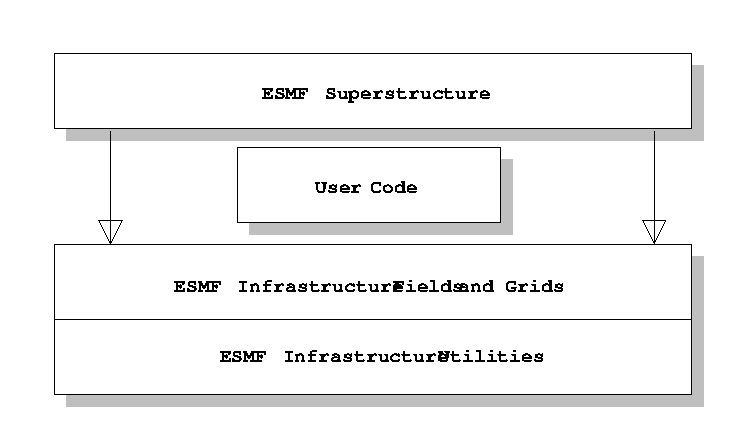
\includegraphics{esmfwich.EPS}}
\end{figure}
\end{center}

\subsection{Programming Paradigm}
A complete, executable assembly of {\bf Superstructure}, user code components and {\bf Infrastructure} collectively forms an ESMF {\it application component}.
Figure \ref{fig:ESMFApplication} shows the generic structure of an ESMF application component. 
This figure shows a single tier composition involving three components. It captures the essence of the composition based programming paradigm that 
ESMF employs, multi-tier composition is also supported in which components are recursively nested.
An application is composed by connecting together one or more
numerical simulation or other user code components within an overall ESMF based environment, figure \ref{fig:ESMFApplication} (1). User code components, figure \ref{fig:ESMFApplication} (3), are written
or modified to fit within the ESMF environment that envelopes
the user code components and that supports a unified high-level {\bf Superstructure} for connecting data and control flows between 
components. A foundation-level {\bf Infrastructure} is also provided, figure \ref{fig:ESMFApplication} (2),
to both accelerate user code development and ensure compatibility
and consistency between components and between hardware platforms. 
\begin{center}
\begin{figure}
\caption{The ESMF programming paradigm defines how an overall application is constructed. An application is an assembly
of one or more gridded and coupler components (1). Components may make use of the ESMF {\bf Infrastructure} toolkit (2). All components,
gridded components, coupler components and the top-level application component are primarily user written (3).}
\label{fig:ESMFApplication}
\scalebox{.5}{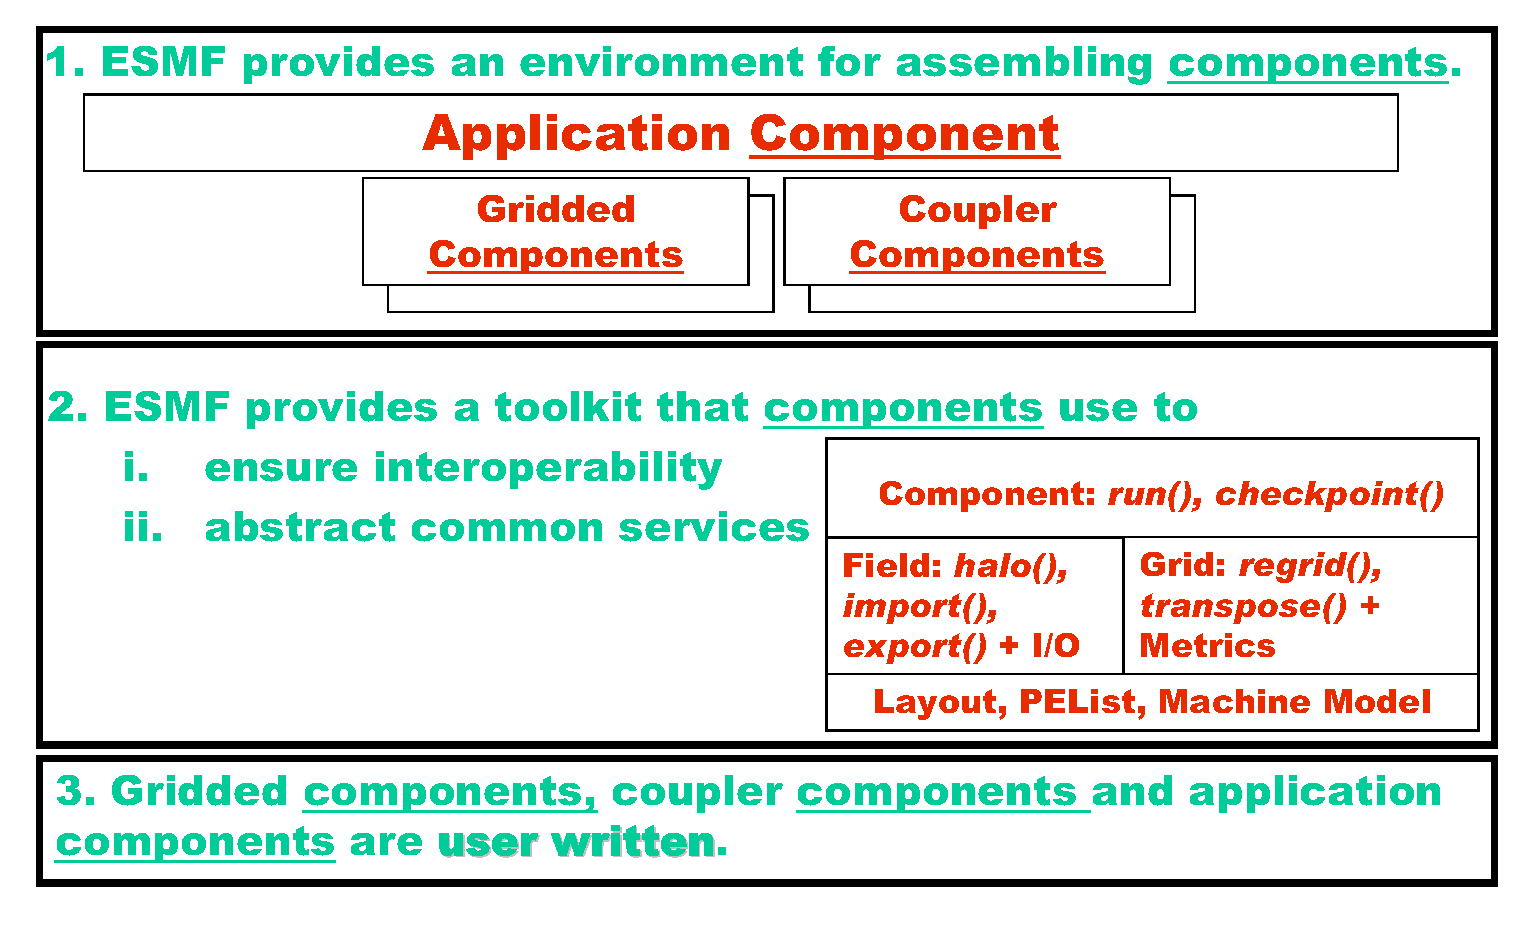
\includegraphics{ESMFprogrammingparadigm.eps}}
\end{figure}
\end{center}

\subsection{Superstructure}
\label{sec:superstructure}
The ESMF {\bf Superstructure} layers in an application furnish a unifying context within which user components are interconnected. For 
example an atmospheric model may use a particular land-surface model in calculating simulated evaporative fluxes. 
The flow of data and sequence of computation between atmospheric model term evaluations and land-surface model
term evaluations would be prescribed in the {\bf Superstructure} layer. Under ESMF user code components are constructed or adapted
to fit within this {\bf Superstructure} layer. This ensures that large components can be interchanged. There may still be issues
of physical consistency between components, but ensuring that all components comply with the requirement to fit
within an ESMF {\bf Superstructure} layer eliminates computational incompatibilities. 

The {\bf Superstructure} layer provides
the foundation for a flexible mechanism to address physical consistency between components that may use different dimensions or units to represent the
same quantity or that may partition physical data differently. Classes called {\it Gridded Components}, 
{\it Coupler Components}, {\it Import States} and {\it Export States} are used within the {\bf Superstructure} layer
to achieve this flexibility.
We describe these classes below:

\subsubsection{Import and Export State Classes}
User code components under ESMF use special interface objects for component to component data exchanges. These objects are 
of type Import State and Export State. These special types support a variety of methods that allow user code components 
to, for example, fill an export state object with data to be shared with other components or query an import state object to 
determine its contents. In keeping with the overall requirements for high-performance it is permitted for Import State and
Export State contents to use references or pointers to component data, so that costly data copies of potentially
very large data structures can be avoided where possible. The content of an Import State and an Export State is 
self-describing, so that different standards can be applied to content labeling depending on the 
by a suite of components.

\subsubsection{Interface Standards}
The Import State and Export State abstractions are designed to be flexible enough
that ESMF does not need to mandate a single standard for fields. For example ESMF does not prescribe the units
of quantities exported or imported, instead it provides mechanics to describe the units, memory layout, grid coordinates 
of the fields in Import States and Export States.  This allows the ESMF software to support a range of different policies for
physical fields. The interoperability experiments that we are using to demonstrate ESMF make use of the emerging
CF standards \cite{ref:CF} for describing physical fields. This is a policy choice for that set of experiments. The ESMF 
software itself can support arbitrary conventions for labeling and characterizing the content of Import and 
Export States.

\subsubsection{Gridded Component Class}
The Gridded Component class is used to for a user component that takes in one Import State and produces one
Export State, both based on the same discrete grid. Examples of Gridded Components are major Earth system 
model components such as land-surface models, ocean models, atmospheric models and sea-ice models. Components 
used for linear algebra manipulations in a state-estimation or data-assimilation optimization procedure are also 
created as Gridded Components. In general the Import State and the Export State of a Gridded Component will 
use the same base discrete grid.

\subsubsection{Coupler Component Class}
The other top-level component class supported in the current ESMF architecture is a Coupler Component class.
This class is used for components that take one or more Import States as input and map them through
spatial and temporal interpolation or extrapolation onto an output Export State. In a Coupler Component
it is often the case that the output Export State is on a different base discrete grid to that of
the Import State(s). The role of Coupler Components is generally mapping the Export States from one or
more Gridded Components to the Import State of another Gridded Component. For example, in a coupled
ocean-atmosphere simulation a Couple Component would be used to map a set of sea-surface fields 
in an ocean model to appropriate planetary boundary layer fields in an atmospheric model.
\subsubsection{Flexible data and control flow}
Import States, Export States, Gridded Components and Coupler Components can be arrayed flexibly
within a {\bf Superstructure} layer. Using these constructs it is possible to configure a set of concurrently
executing Gridded Components joined through a single Coupler Component of the style shown in figure 
\ref{fig:hubspoke}. Is is also possible to configure a set of sequentially executing components with multiple
pair-wise Coupler Components defined to support individual Gridded Component to Gridded 
Component mappings independently, figure \ref{fig:point2point}.

\begin{figure}
\caption{ESMF can support configurations with a single central Coupler Component. In this case inputs from all Gridded 
Components are transferred and regrided between all components in one place. The block arrows show how the 
Coupler Component 
(symbolized by the star icon) must take inputs from all Gridded Components (symbolized by the model output images) 
and return data to all Gridded Components.}
\label{fig:hubspoke}
\scalebox{0.7}{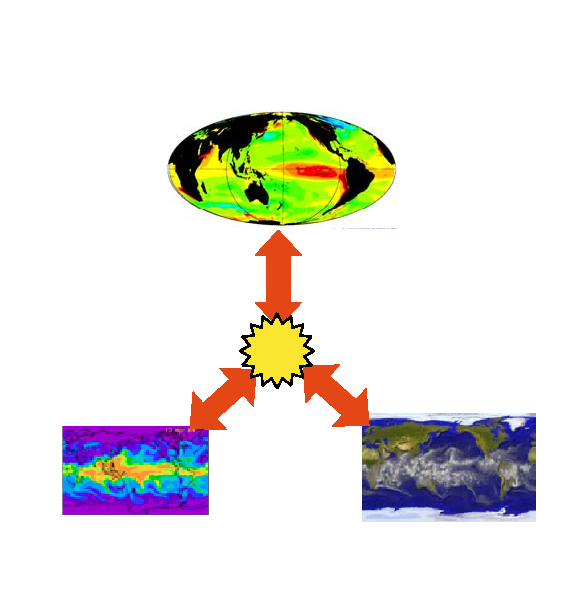
\includegraphics{couplings_hub_and_spoke.eps}}
\end{figure}

\begin{figure}
\caption{ESMF also supports configurations with multiple point to point Coupler Components. 
These take inputs from one Gridded
Component and transfer and regrid the data for passing to another Gridded Component. The block arrows show the
flow of data between point to point pairings of Coupler Components (symbolized by the star icons) and Gridded 
Components (symbolized by the model output images).}
\label{fig:point2point}
\scalebox{0.7}{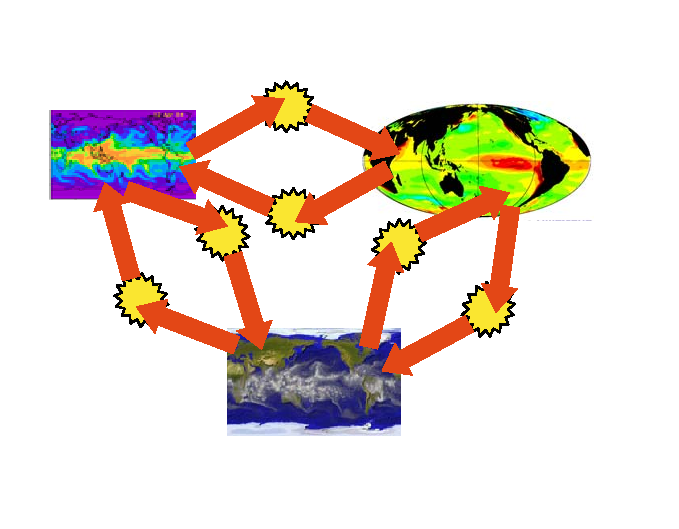
\includegraphics{couplings_pt_to_pt.eps}}
\end{figure}

The set of {\bf Superstructure} abstractions allows flexible data-flow and control between components. However, 
components will often use different discrete grids, and time-stepping components may march forward with different time
intervals. In a parallel compute environment different components may be distributed in a different manner on the
underlying compute resources. The ESMF {\bf Infrastructure} layer provides elements to manage this complexity.

\subsection{Infrastructure}
\label{sec:infrastructure}
Figure \ref{fig:threecomponents} illustrates three Gridded Components that use three different grids being coupled together. In 
order to achieve this coupling several steps beyond defining {\bf Superstructure} Import State and Export State objects to act
as data conduits are required. Coupler Components are required that can map between the different
grids, this mapping may also involve mapping between different units and/or memory layout conventions for the fields that
pass between components. In a parallel compute environment the Coupler Components may also be required to map between different 
domain decompositions. In order to advance in time correctly the separate Gridded Components must have compatible notions
of time. Approaches to parallelism within the Gridded Components must also be compatible. The {\bf Infrastructure} layer
contains a set of classes that address these issues and assist in managing overall system complexity. We describe
these classes below:

\begin{figure}
\caption{Schematic showing the coupling of components that use different discrete grids and different time-stepping. 
In this example component {\it NCAR Atmosphere} might use a spectral grid based on spherical harmonics, component
{\it GFDL Ocean} might use a latitude-longitude grid but with a patched decomposition that does not include
land masses and component {\it NSIPP Land} might use a mosaic based grid for representing vegetation patchiness
and a catchment area based grid for river routings. The {\bf Infrastructure} layer contains tools to help develop 
software for coupling between components on different grids, mapping between components with different distributions in a 
multi-processor compute environment and to synchronize events between components with different time-stepping intervals 
and algorithms.  }
\label{fig:threecomponents}
\scalebox{0.5}{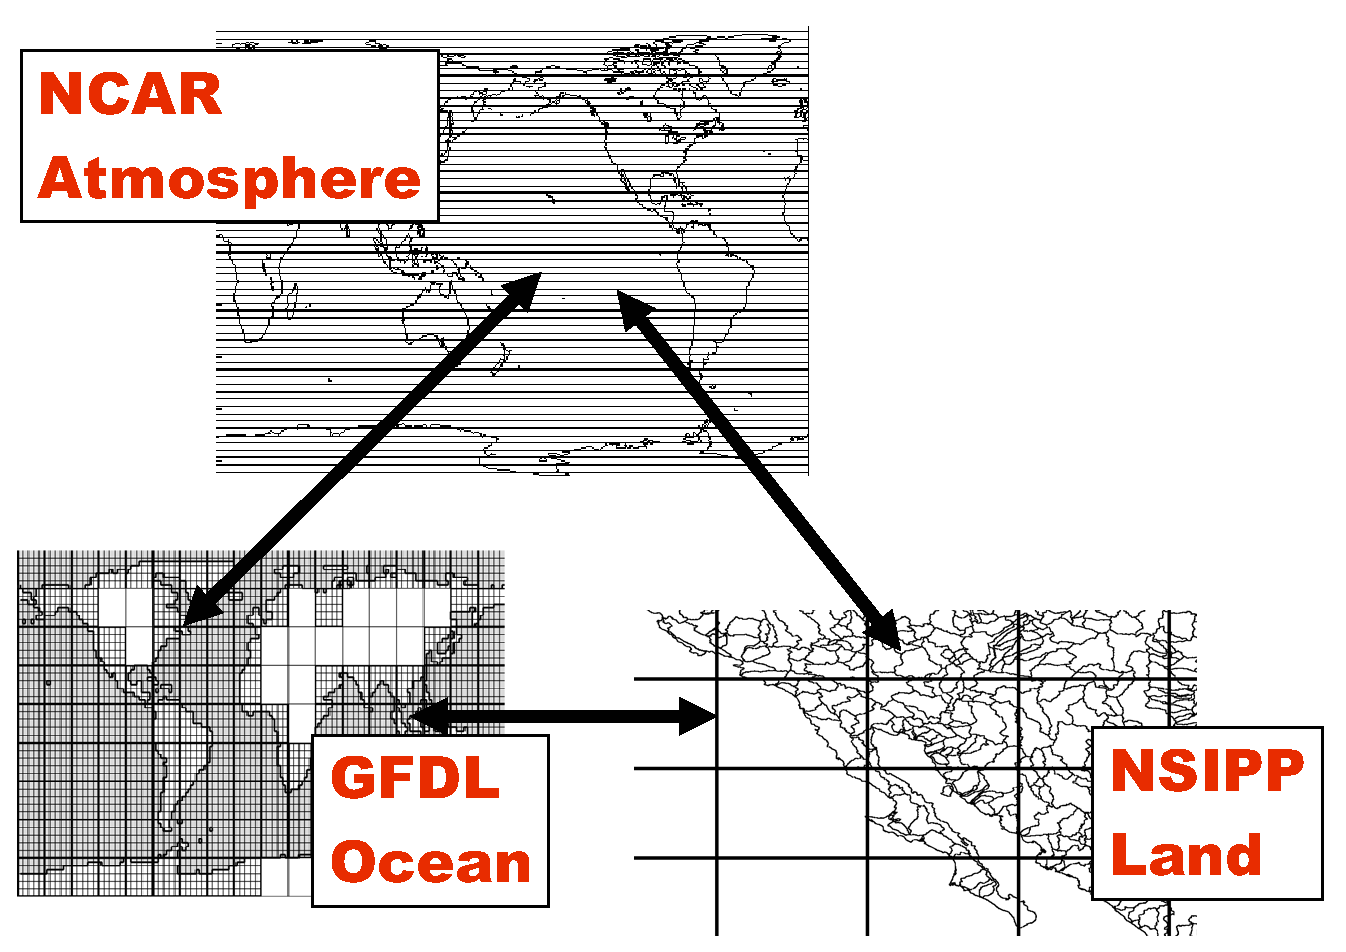
\includegraphics{regrid.eps}}
\end{figure}

\subsubsection{Field and Array Classes}
The {\it Field} and {\it Array} classes contain data together with descriptive
physical and computational attribute information. The physical attributes include information that describes the units
of the data. The computational attributes include information on the layout in memory of the field data. The Field class
is primarily geared toward structured data. A comparable class called {\it Location Stream} provides a self-describing
container for unstructured observational data streams.

\subsubsection{Physical Grid Class}
The {\it Physical Grid} class is an extensible class that holds discrete grid information. It has subtypes that allow
it to serve as a container for the full range of different physical grids that might arise in a coupled system.
In the example in figure \ref{fig:threecomponents} objects of type Physical Grid would hold grid information for
each of the spectral grid, the latitude-longitude grid, the mosaic grid and the catchment grid. 

\subsubsection{Regrid Class}
The {\it Regrid} class is an extensible class that allows conservative remapping between a field on one physical grid
to a field on a different physical grid \cite{ref:SCRIP}. It supports precomputation of grid interpolation weights and allows user selectable
corrections for global or local conservation requirements. Regrid is designed to be scalable on parallel platforms.
When mapping between grids
the Regrid class utilizes the Physical Grid object and Field and Array objects.

\subsubsection{Distributed Grid Class}
The {\it Distributed Grid} class is used to represent the decomposition of a data structure into sub-domains, typically for
parallel processing purposes. The class is designed to support a generalized ``ghosting'' for tiled 
decompositions of finite difference, finite volume and finite element codes. 

\subsubsection{Time and Calendar Management Class}
To support synchronization between components {\it Time} and {\it Calendar} classes along with an associated
{\it Clock} class are provided. These classes allow Gridded and Coupler Component processing
to be latched to a common controlling clock.

\subsubsection{I/O Classes}
The {\bf Infrastructure} layer defines a set of {\it I/O} classes for storing and retrieving Field and Grid information
to and from persistent storage. The I/O classes support a range of standard formats including binary I/O and netCDF, HDF5 and
GRIB based I/O.

\subsubsection{Communication Class}
To provide a mechanism for ensuring performance portability ESMF defines a {\it Communication} class. This class provides a set of
high-level platform independent interfaces to performance critical parallel processing communication routines. These routines can be tuned
to specific platforms to ensure optimal parallel performance on many platforms. The Communication class includes reduction
operations, transpose or redistribution operations and halo or ghost operations.

\subsubsection{Logging and Profiling Class}
The {\it Logging} and {\it Profiling} classes are designed to aid in managing the complexity of multi-component applications. They provide
ESMF with a unified mechanism for notification messages, for timing and counting events.







% $Id: ESMF_usrdoc.tex,v 1.21 2003/05/07 22:43:12 cdeluca Exp $





\bodytext{BGCOLOR=white LINK=#083194 VLINK=#21004A}



%\section{Introduction}


\section{ESMF\_COUPLED\_FLOW Demonstration Program}
\label{sec:demo}

\subsection{Introduction}

This section describes the organization of a
demonstation program which uses the ESMF Framework,
including use of both the 
Superstructure and Infrastructure.

\subsection{ESMF\_COUPLED\_FLOW Description}
 
The {\tt ESMF\_COUPLED\_FLOW} application is comprised of two ESMF 
{\tt Gridded Components} and a {\tt Coupler Component}.  
The first {\tt Gridded Component}, {\tt FlowSolver}, solves the compressible 
time-dependent fluid flow equations.  The algorithm 
applies an explicit solution technique to a staggered, Arakawa C igrid 
that is cartesian and uniform.  State variables, including density, 
pressure, viscosity and temperature, are located at cell-centers, while 
velocities are located at cell faces.  This component is initialized 
with a steady-state, one-dimensional flow.  The second {\tt Gridded 
Component}, {\tt Injector}, injects fluid into the first normal to the 
flow along 
one of the boundaries.  The injected fluid can have arbitrary velocity, 
temperature, density and duration, effectively setting some of 
the boundary conditions for the first component.  The {\tt FlowSolver} and 
{\tt Injector Components} sit on different cartesian igrids.  The
{\tt Coupler Component} redistributes boundary condition data from 
the {\tt Injector} to the {\tt FlowSolver}.





%\section{Major Pieces}


\section{Program Organization}

The demonstration program consists of a top level Application
Driver, a top level Gridded Component, and nested within this Gridded
Component are 3 subcomponents: a Coupler Component and 2 Gridded Components.

The following diagram shows this organization.  Note that there
is no direct communication between the subcomponents; all
interactions are mediated by the top level Gridded Component.

Each component communicates via Initialize, run, and finalize
subroutine calls.  These go through the ESMF where
they are checked for validity, default values are supplied,
and only those components involved in the computation are
invoked.

% the bpht says we prefer the bottom of a page, then separate page,
% then here, then top last.

\begin{figure}[bpht]
\caption[Components]{Structure of the demonstration program.}
\label{fig:democomps}
\begin{center}
\scalebox{0.70}{\includegraphics{ESMMF_demo.eps}}
\end{center}
\end{figure}





\section{Framework Usage Details}


\input{../Demo/coupled_flow/doc/CoupledFlowApp_fapi}



\input{../Demo/coupled_flow/doc/CoupledFlowDemo_fapi}



\input{../Demo/coupled_flow/doc/FlowSolverMod_fapi}



\input{../Demo/coupled_flow/doc/FlowArraysMod_fapi}



\input{../Demo/coupled_flow/doc/CouplerMod_fapi}



\input{../Demo/coupled_flow/doc/InjectorMod_fapi}



\input{../Demo/coupled_flow/doc/InjectArraysMod_fapi}


%\subsubsection{Restrictions}
%#ifdef STANDALONE
%\input{flow_res}
%#elif defined(1 )
%\input{../Demo/coupled_flow/doc/flow_res}
%#endif


%#ifdef STANDALONE
%\section{Review Status}
%\input{flow_rev}
%#endif

%#ifdef STANDALONE
%\section{Glossary}
%\input{flow_glos}
%#endif






%\section{ESMF Technical Overview}
% $Id$

\section{Compiling and Linking User Code against an ESMF Installation}
\label{sec:Use}
% $Id: ESMF_use.tex,v 1.33 2010/10/28 23:37:15 theurich Exp $

Building user applications against an ESMF installation requires that the 
compiler and linker be able to find the appropriate ESMF header, module and 
library files. If this procedure has been documented by the installer of the 
ESMF library on your system then follow the directions given. Otherwise it is up 
to the user to determine and provide the required compiler and linker flags. 
Every ESMF installation provides a file named {\tt esmf.mk} that contains the 
relevant information.

The location of the {\tt esmf.mk} file should be documented by the party that 
installed ESMF on the system. We recommend that a single ESMF specific 
environment variable, {\tt ESMFMKFILE}, be provided by the system that points to 
the {\tt esmf.mk} file. See section \ref{InstallESMF} for the related discussion 
aimed at the person that installs ESMF on a system.

The information in {\tt esmf.mk} is defined in form of variables. In fact, 
syntactically {\tt esmf.mk} is a makefile fragment and can be imported by an 
application specific makefile via the {\tt include} command. All the variables 
in {\tt esmf.mk} start with the "{\tt ESMF\_}" prefix to prevent conflicts. The 
information in {\tt esmf.mk} is fully specified and is not affected by any 
variables set in the user's environment.

The information defined in {\tt esmf.mk} includes Fortran compiler and linker, 
as well as C++ compiler and linker. It further includes the recommended Fortran 
and C++ specific compiler and linker flags for building ESMF applications. One 
way of using the {\tt esmf.mk} is to glean the necessary information from it. 
This information can then be used either directly on the command line when 
compiling a user application, or to hardwire the settings into the application 
specific build system. However, the recommended use of {\tt esmf.mk} is to 
include this file in the application specific makefile directly via the 
{\tt include} command.

The {\tt Makefile} template below demonstrates how a user build system can be 
constructed to leverage the {\tt esmf.mk} file. In practice, most user build 
systems will be more complex. However, this template does show that the added 
complexity introduced by using {\tt esmf.mk} is minimal. Examples of how to use 
this build system in realistic user scenarios can be found in the 
\htmladdnormallink{external demos}{http://www.earthsystemmodeling.org/users/code_examples/external_demos/external_demos.shtml}.

The advantages of using {\tt esmf.mk}, over hard coding suitable compiler and 
linker flags into the user build system directly, are robustness and portability. 
Robustness is a consequence of the fact that everything defined in {\tt esmf.mk} 
corresponds to the exact settings used during the ESMF library build 
(consistency) and during the ESMF test suite build. Using {\tt esmf.mk} thus 
guarantees that the user application is build in the exact same manner as the 
ESMF test suite applications that undergo strict regression testing before every 
ESMF release. Portability means that a user build system, which uses 
{\tt esmf.mk} in the way the template {\tt Makefile} demonstrates, will function 
as expected on any system where ESMF was successfully installed and tested, 
without the need of modifying anything. Every {\tt esmf.mk} is generated during 
a specific ESMF installation using the ESMF tested settings for the host 
platform.

\begin{verbatim}

################################################################################
### Makefile template for user ESMF application, leveraging esmf.mk mechanism ##
################################################################################

################################################################################
### Finding and including esmf.mk ##############################################

# Note: This fully portable Makefile template depends on finding environment
#       variable "ESMFMKFILE" set to point to the appropriate "esmf.mk" file,
#       as is discussed in the User's Guide.
#       However, you can still use this Makefile template even if the person
#       that installed ESMF on your system did not provide for a mechanism to
#       automatically set the environment variable "ESMFMKFILE". In this case
#       either manually set "ESMFMKFILE" in your environment or hard code the
#       location of "esmf.mk" into the include statement below.
#       Notice that the latter approach has negative impact on portability.

ifneq ($(origin ESMFMKFILE), environment)
$(error Environment variable ESMFMKFILE was not set.)
endif

include $(ESMFMKFILE)

################################################################################
### Compiler and linker rules using ESMF_ variables supplied by esmf.mk ########

.SUFFIXES: .f90 .F90 .c .C

.f90:
	$(ESMF_F90COMPILER) -c $(ESMF_F90COMPILEOPTS) $(ESMF_F90COMPILEPATHS) \
          $(ESMF_F90COMPILEFREENOCPP) $<
	$(ESMF_F90LINKER) $(ESMF_F90LINKOPTS) $(ESMF_F90LINKPATHS) \
          $(ESMF_F90LINKRPATHS) -o $@ $*.o $(ESMF_F90ESMFLINKLIBS)        

.F90:
	$(ESMF_F90COMPILER) -c $(ESMF_F90COMPILEOPTS) $(ESMF_F90COMPILEPATHS) \
          $(ESMF_F90COMPILEFREECPP) $(ESMF_F90COMPILECPPFLAGS) $<
	$(ESMF_F90LINKER) $(ESMF_F90LINKOPTS) $(ESMF_F90LINKPATHS) \
          $(ESMF_F90LINKRPATHS) -o $@ $*.o $(ESMF_F90ESMFLINKLIBS)        
        
.c:
	$(ESMF_CXXCOMPILER) -c $(ESMF_CXXCOMPILEOPTS) \
          $(ESMF_CXXCOMPILEPATHSLOCAL) $(ESMF_CXXCOMPILEPATHS) \
          $(ESMF_CXXCOMPILECPPFLAGS) $<
	$(ESMF_CXXLINKER) $(ESMF_CXXLINKOPTS) $(ESMF_CXXLINKPATHS) \
          $(ESMF_CXXLINKRPATHS) -o $@ $*.o $(ESMF_CXXESMFLINKLIBS)

.C:
	$(ESMF_CXXCOMPILER) -c $(ESMF_CXXCOMPILEOPTS) \
          $(ESMF_CXXCOMPILEPATHSLOCAL) $(ESMF_CXXCOMPILEPATHS) \
          $(ESMF_CXXCOMPILECPPFLAGS) $<
	$(ESMF_CXXLINKER) $(ESMF_CXXLINKOPTS) $(ESMF_CXXLINKPATHS) \
          $(ESMF_CXXLINKRPATHS) -o $@ $*.o $(ESMF_CXXESMFLINKLIBS)

################################################################################
### Sample targets for user ESMF applications ##################################

all: esmf_UserApplication esmc_UserApplication

esmf_UserApplication:

esmc_UserApplication:

################################################################################

\end{verbatim}


\section{Using Bundled ESMF Applications}
\label{sec:Apps}
% $Id: ESMF_apps.tex,v 1.8 2010/10/28 23:37:15 theurich Exp $

ESMF comes with a set of bundled applications in the form of standard command 
line tools. These applications include convenient access to general information 
about an ESMF installation, and regrid weight file generation (sometimes
referred to as "offline" regridding). This section provides assistance with
respect to building and running the bundled applications. If you are using a
pre-installed ESMF on your system, follow the local instructions provided by
the installer or system admin of how to access and run the ESMF applications.
Often access is as simple as loading a configuration module to have the
correct path to the ESMF application binaries added to your {\tt PATH}
environment variable.

There are two ways a user may choose to build and access the bundled ESMF 
applications. Users that prefer not to go through the full ESMF installation 
process have the option to build the bundled applications inside of the ESMF 
source tree, very similar to how the unit tests, system tests and examples are 
built. This option is outlined in section \ref{quickapps} and should only be 
considered by users that want quick access to the applications and are not 
interested in a sharable installation or the development of portable scripts and 
makefiles that use the applications. Users interested in the latter should 
consider the more standard second option outlined below.

The bundled ESMF applications are built automatically in the process of 
installing ESMF following the instructions given in section \ref{InstallESMF}. 
On systems that offer system-wide ESMF installations (e.g. via modules or 
similar mechanisms) the user need not worry about the build and installation 
details. Once installed, the applications are accessible through their precise 
location on the system. For this purpuse every ESMF installation provides a file 
named {\tt esmf.mk} that contains the variable {\tt ESMF\_APPSDIR} which 
specifies the precise application path.

The {\tt esmf.mk} mechanism used for application access is the same as the one 
described in section \ref{sec:Use} for writing robust and portable user 
makefiles for building and linking user applications against an ESMF 
installation. One feature of the {\tt esmf.mk} mechanism is that only one single 
piece of information must be known about an ESMF installation to use it, and 
that is the location of file {\tt esmf.mk} itself. The location of this file 
should be documented by the party that installed ESMF on the system. We 
recommend that a single ESMF specific environment variable ESMFMKFILE be 
provided by the system that points to the {\tt esmf.mk} file. See section 
\ref{InstallESMF} for the related discussion aimed at the person that installs 
ESMF on a system.

Once the exact location of the bundled ESMF application files has been 
determined, either by inspecting the associated {\tt esmf.mk} file, or by using 
the {\tt ESMF\_APPSDIR} makefile variable directly in the user script or 
makefile, the applications can be executed following the system specific rules 
for execution. The details will depend on whether ESMF was built with or without 
MPI dependency. In the latter case the system specific rules for launching 
parallel applications must be followed. System specific execution details on 
this level are outside of ESMF's scope. However, ESMF does offer specific 
application use examples as part of the {\it external\_demos} module described 
online at the 
\htmladdnormallink{External Demos webpage}{http://www.earthsystemmodeling.org/users/code_examples/external_demos/external_demos.shtml}. 
For most systems, the MPI version of the ESMF bundled applications can be 
executed by a command equivalent to:

\begin{verbatim}

mpirun -np X $(ESMF_APPSDIR)/application

\end{verbatim}
 
where {\tt X} specifies the total number of PETs and {\tt application} is the 
name of the specific ESMF application to be executed.
 
All bundled ESMF applications support the standard \verb+ '--help'+ command line 
option that prints out information on its proper use.  More detailed 
instructions of the individual applications are available in the "Applications" 
section of the {\it ESMF Reference Manual}.


\newpage

\section{Building and Installing the ESMF}
\label{sec:TechOver}

This section goes into more detail about how to build and install the ESMF
software.

% $Id$

%\section{Building and Installing the ESMF}
\subsection{ESMF Download Options}

Major releases of the ESMF software can be downloaded by following
the instructions on the the {\bf Download} link on the ESMF 
website, \htmladdnormallink{http://www.earthsystemmodeling.org}{http://www.earthsystemmodeling.org}.

The ESMF is distributed as a full source code tree.
Follow the instructions in the following sections
to build the library and link it with your application.

\subsection{Acquiring Development Snapshots}
Occasionally, it is helpful to acquire a development snapshot of ESMF
in order to test emerging capabilities, optimizations, and bug fixes
before they are available in a formal release.  Development snaphots
are ``use at your own risk.'' Efforts are made to ensure that most unit
and system tests are passing on typical platforms, but there are no
guarantees of the stability of development snapshots. New APIs available
in development snapshots may change before the next release.

Users aware of these risks may check out development snapshots
using the appropriate git tag.  The standard naming convention
for development tags is:

\begin{verbatim}
ESMF_<VERSION>_beta_snapshot_<NUMBER>
\end{verbatim}

For example, to check out ESMF version 7.1.0 beta snapshot 31, use the
following command:

\begin{verbatim}
  $ git archive --remote=git://git.code.sf.net/p/esmf/esmf --format=tar --prefix=esmf/ ESMF_7_1_0_beta_snapshot_31 | tar xf -
\end{verbatim}

Once downloaded, development snapshots are built in the same way as releases.

\subsection{System Requirements}
\label{sec:systemreq}
% $Id$


The following compilers and utilities are required for compiling, linking and
testing the ESMF software:
\begin{itemize}
\item Fortran90 (or later) compiler;
\item C++ compiler;
\item MPI implementation compatible with the above compilers (but see below);
\item GNU's \htmladdnormallink{gcc compiler}{http://gcc.gnu.org} -
for a standard cpp preprocessor implementation;
\item \htmladdnormallink{GNU Make}{http://www.gnu.org/software/make/make.html}; 
\item \htmladdnormallink{Perl}{http://www.perl.com/download.csp} - for running
test scripts.
\end{itemize} 

Internal packages that can optionally reference external libraries:
\begin{itemize}
\item LAPACK - version 3.x or newer
\item ParallelIO (PIO) - version 2.5.7 or newer
\item yaml-cpp - tag yaml-cpp-0.6.2 or newer
\end{itemize}

Optional external packages that must be specified for certain functions:
\begin{itemize}
\item NetCDF - version 3.6.x or newer (version 4.4 or newer required by PIO)
\item parallel-NetCDF - version 1.2.0 or newer (version 1.12 or newer required by PIO)
\item Xerces - version 3.1.0 or newer
\end{itemize}  

ESMF can be built using a single-processor MPI-bypass library
that comes with ESMF by setting {\tt ESMF\_COMM=mpiuni}. This allows ESMF applications
to be linked and run in single-process mode.

In order to build html and pdf versions of the ESMF documentation, 
\htmladdnormallink{\LaTeX}{http://www.latex-project.org},
the \htmladdnormallink{latex2html}{http://www.latex2html.org}
conversion utility, and the Unix/Linux {\tt dvipdf} utility must be installed.
The csh shell is also required to complete the documentation build.


\subsection{Third Party Libraries}
\label{sec:ThirdParty}

Some portions of the ESMF library can offer enhanced capabilities when
certain third party libraries are available. This section describes
these dependencies and the associated environment settings
that allow the user to control them.

On many platforms, the ESMF library is also created as a shared library.
When third party libraries are called from ESMF, it is recommended that they are
also available as shared libraries.  In cases where they are not, they should at
least be compiled with the position independent code option enabled (e.g., -fPIC on
Linux with gfortran/gcc) where necessary, so that the ESMF shared library
build can successfully incorporate them.

\subsubsection{LAPACK}
\label{sec:lapack}
The patch recovery regridding method of the ESMF Mesh class requires solving
local least squares problems. It uses the
\htmladdnormallink{LAPACK}{http://www.netlib.org/lapack} {\it DGELSY} solver 
to carry out this task.

The following environment variables control whether a minimal set of
LAPACK code that comes with ESMF is used, or whether ESMF should link against
an externally available LAPACK installation. Alternatively, ESMF's
LAPACK-dependent features can be turned off altogether.

\begin{description}

\item[ESMF\_LAPACK] Possible value: {\tt "internal"} (default), {\tt "OFF"},
 {\tt "system"}, {\tt "mkl"}, {\tt "netlib"}, {\tt "scsl"}, {\it <userstring>}.

\begin{description}
\item[{\tt "internal"} (default)] ESMF will be compiled with LAPACK-dependent
features. A minimal set of LAPACK/BLAS code included in ESMF will be used
to satisfy the dependencies.

\item[{\tt "OFF"}] Disables LAPACK-dependent code.
 
\item[{\tt "system"}] A system-dependent external LAPACK/BLAS installation
is used to satisfy the external dependencies of the LAPACK-dependent ESMF code.
Sets {\tt ESMF\_LAPACK\_LIBS} appropriately.

\item[{\tt "mkl"}] The Intel MKL library is used to satisfy the external 
dependencies of the LAPACK-dependent ESMF code. When {\tt ESMF\_COMPILER} is set to
{\tt "intel"}, {\tt ESMF\_LAPACK\_LIBS} is set to {\tt "-mkl"}.  Otherwise {\tt ESMF\_LAPACK\_LIBS}
is set to {\tt "-lmkl\_lapack -lmkl"}, unless it is already defined in the user 
environment.

\item[{\tt "netlib"}] The NETLIB library is used to satisfy the external 
dependencies of the LAPACK-dependent ESMF code. Sets {\tt ESMF\_LAPACK\_LIBS} to
{\tt "-llapack -lblas"}, unless it is already defined in the user environment.

\item[{\tt "scsl"}] The SCSL library is used to satisfy the external 
dependencies of the LAPACK-dependent ESMF code. Sets {\tt ESMF\_LAPACK\_LIBS} to
{\tt "-lscs"}, unless it is already defined in the user environment.

\item[{\it <userstring>}] Enables ESMF's LAPACK-dependent code, but does not set
a default for {\tt ESMF\_LAPACK\_LIBS}.  {\tt ESMF\_LAPACK\_LIBS}, and if 
required, {\tt ESMF\_LAPACK\_LIBPATH}, must be set explicitly in the user 
environment.
\end{description}

\item[ESMF\_LAPACK\_LIBPATH] Typical value: {\tt /usr/local/lib} (no default).

Specifies the path where the LAPACK library is located.

\item[ESMF\_LAPACK\_LIBS] Typical value: {\tt "-llapack -lblas"} 
(default is dependent on {\tt ESMF\_LAPACK}).

Specifies the linker directive needed to link the LAPACK library to
the application.  On some systems, the BLAS library must also be included.
\end{description}


\subsubsection{NetCDF}
\label{sec:netcdf}
ESMF provides the ability to read Grid and Mesh data in 
\htmladdnormallink{NetCDF}{http://www.unidata.ucar.edu/software/netcdf/} format. 

Beginning with NetCDF 4.2, the C and Fortran API libraries are released as separate packages.
To compile ESMF with NetCDF 4.2 and newer releases, the {\tt ESMF\_NETCDF} environment variable
can be set to {\tt "split"}.  The {\tt "split"} option requires the NetCDF C library, 
and the NetCDF Fortran API library be installed in the same directory.  As an alternative,
the {\tt "nc-config"} option may be used to automatically determine the include and lib directory
locations.  The {\tt "nc-config"} option supports separate C and Fortran directories.


The following environment variables enable, and specify the name and location
of the desired NetCDF library and associated header files:

\begin{description}

\item[ESMF\_NETCDF] Possible value: {\it not set} (default), {\tt "nc-config"}, {\tt "split"}, 
{\tt "standard"}, {\it <userstring>}.

\begin{description}
\item[{\it not set}] (default) NetCDF-dependent features will be disabled.
The {\tt ESMF\_NETCDF\_INCLUDE}, {\tt ESMF\_NETCDF\_LIBPATH}, and
{\tt ESMF\_NETCDF\_LIBS} environment variables will be ignored.

\item[{\tt "nc-config"}] The NetCDF {\tt nc-config} and if available, {\tt nf-config},
tools will be used to determine the proper settings of {\tt ESMF\_NETCDF\_INCLUDE},
{\tt ESMF\_NETCDF\_LIBPATH}, and {\tt ESMF\_NETCDF\_LIBS}.  The shell {\tt PATH}
environment variable must include the NetCDF bin directories where {\tt nc-config}
and {\tt nf-config} reside.  This option supports having the main NetCDF library and the
Fortran API library reside in separate directories.

\item[{\tt "split"}] {\tt ESMF\_NETCDF\_LIBS} will be set to 
{\tt "-lnetcdff -lnetcdf"}.  This option is useful for systems 
which have the Fortran and C bindings archived in separate library files.  
The {\tt ESMF\_NETCDF\_INCLUDE} and {\tt ESMF\_NETCDF\_LIBPATH}
environment variables will also be used, if defined.

\item[{\tt "standard"}] {\tt ESMF\_NETCDF\_LIBS} will be set to 
{\tt "-lnetcdf"}.  This option is useful when the Fortran and 
C bindings are archived together in the same library file.  The {\tt ESMF\_NETCDF\_INCLUDE} 
and {\tt ESMF\_NETCDF\_LIBPATH} environment variables will also be used, 
if defined.

\item[{\it <userstring>}] If set, {\tt ESMF\_NETCDF\_INCLUDE}, 
{\tt ESMF\_NETCDF\_LIBPATH}, and {\tt ESMF\_NETCDF\_LIBS} environment 
variables will be used, if defined.
\end{description}

\item[ESMF\_NETCDF\_INCLUDE] Typical value: {\tt /usr/local/include} 
(no default).

Specifies the path where the NetCDF header files are located.

\item[ESMF\_NETCDF\_LIBPATH] Typical value: {\tt /usr/local/lib} (no default).

Specifies the path where the NetCDF library file is located.

\item[ESMF\_NETCDF\_LIBS] Typical value: {\tt "-lnetcdf"} 

Specifies the linker directives needed to link the NetCDF library to
the application.

The default value depends on the setting of {\tt ESMF\_NETCDF}.  For the 
typical case where {\tt ESMF\_NETCDF} is set to {\tt "standard"}, 
{\tt ESMF\_NETCDF\_LIBS} is set to {\tt "-lnetcdf"}.  
When {\tt ESMF\_NETCDF} is set to {\tt "split"}, {\tt ESMF\_NETCDF\_LIBS} 
is set to {\tt "-lnetcdff -lnetcdf"}.

If the hdf5 library is required, append {\tt "-lhdf5\_hl -lhdf5"} to the
desired setting.  E.g. {\tt "-lnetcdff -lnetcdf -lhdf5\_hl -lhdf5"}
\end{description}

\subsubsection{Parallel-NetCDF}
\label{sec:pnetcdf}
ESMF provides the ability to write Mesh weights using 
\htmladdnormallink{Parallel-NetCDF}{http://trac.mcs.anl.gov/projects/parallel-netcdf}.

Some file systems, for example \htmladdnormallink{Lustre}{http://wiki.lustre.org}, may need
to have locking attributes enabled when the file system is mounted.

The following environment variables enable and specify the name and 
location of the desired Parallel-NetCDF library and associated header files:

\begin{description}
\item[ESMF\_PNETCDF] Possible value: {\it not set} (default), {\tt "pnetcdf-config"},
{\tt "standard"}, {\it <userstring>}.  

When defined, enables the use of Parallel-NetCDF.

\begin{description}
\begin{sloppypar}
\item[{\it not set}] (default) PNETCDF-dependent features will be disabled.
The {\tt ESMF\_PNETCDF\_INCLUDE}, {\tt ESMF\_PNETCDF\_LIBPATH}, and
{\tt ESMF\_PNETCDF\_LIBS} environment variables will be ignored.
\end{sloppypar}

\item[{\tt "pnetcdf-config"}] The PNetCDF {\tt pnetcdf-config} tool will be used
to determine the proper settings of {\tt ESMF\_PNETCDF\_INCLUDE},
{\tt ESMF\_PNETCDF\_LIBPATH}, and {\tt ESMF\_PNETCDF\_LIBS}.  The shell {\tt PATH}
environment variable must include the PNetCDF bin directory where {\tt pnetcdf-config}
resides.

\item[{\tt "standard"}] {\tt ESMF\_PNETCDF\_LIBS} will be set to 
{\tt "-lpnetcdf"}.  The {\tt ESMF\_PNETCDF\_INCLUDE} and 
{\tt ESMF\_PNETCDF\_LIBPATH} environment variables will also be used, 
if defined.

\item[{\it <userstring>}] If set, {\tt ESMF\_PNETCDF\_INCLUDE},
{\tt ESMF\_PNETCDF\_LIBPATH}, and {\tt ESMF\_PNETCDF\_LIBS} environment
variables will be used.
\end{description}

\item[ESMF\_PNETCDF\_INCLUDE] Typical value: {\tt /usr/local/include} 
(no default).

Specifies the path where the Parallel-NetCDF header files are located.

\item[ESMF\_PNETCDF\_LIBPATH] Typical value: {\tt /usr/local/lib} (no default).

Specifies the path where the Parallel-NetCDF library file is located.

\item[ESMF\_PNETCDF\_LIBS] Typical value: {\tt "-lpnetcdf"}.

Specifies the linker directives needed to link the Parallel-NetCDF library to the
application.
\end{description}

\subsubsection{PIO}
\label{sec:pio}
ESMF provides the ability to read and write data in both binary and 
NetCDF formats through \htmladdnormallink{ParallelIO (PIO)}
{http://code.google.com/p/parallelio/}, a third-party I/O software
library that is integrated in the ESMF library. The following environment
variable enables PIO functionalities inside of ESMF.

The PIO code depends on MPI I/O support by the underlying MPI
implementation to provide the binary format. Almost all current MPI
implementations support MPI I/O to the required degree. For NetCDF format
support the integrated PIO code depends on {\tt ESMF\_PNETCDF}
(see \ref{sec:pnetcdf}) and/or {\tt ESMF\_NETCDF} (see \ref{sec:netcdf})
being enabled.

\begin{description}
\item[ESMF\_PIO] Possible value: {\it not set} (default), {\tt "internal"}.

\begin{description}
\item[{\it not set}] (default) PIO-dependent features will be enabled on platforms where
certain Fortran-2003 C Interoperability features are available.  Most currently supported
compilers support these features.

\item[{\tt "OFF"}] Disables PIO-dependent code.

\item[{\tt "internal"}] PIO-dependent features will be enabled and will use the 
PIO library that is included and built with ESMF.  

\end{description}

\end{description}

\subsubsection{Accelerator Software Stacks}
\label{sec:acc}
ESMF provides the ability to query various third party accelerator software
stacks and gather information about the accelerator devices available in a
system. The users can query the number of accelerator devices accessible
from a PET using the OpenCL, OpenACC, Intel MIC and OpenMP software stacks.

The following environment variables enable, and specify the name and location
of the desired accelerator software stacks and associated header files:

\begin{description}

\item[ESMF\_ACC\_SOFTWARE\_STACK] Possible value: 
{\it not set} (default), {\tt "opencl"}, {\tt "openacc"},
{\tt "intelmic"}, {\tt "openmp4"}.

\begin{description}
\item[{\it not set}] (default) All accelerator software stack related features
 will be disabled.
The {\tt ESMF\_ACC\_SOFTWARE\_STACK\_INCLUDE}, 
{\tt ESMF\_ACC\_SOFTWARE\_STACK\_LIBPATH}, and
{\tt ESMF\_ACC\_SOFTWARE\_STACK\_LIBS} environment variables will be ignored.

\item[{\tt "opencl"}] The ESMF library will use the OpenCL
framework to query information about accelerator devices in the system.
The {\tt ESMF\_ACC\_SOFTWARE\_STACK\_INCLUDE},
{\tt ESMF\_ACC\_SOFTWARE\_STACK\_LIBPATH} and
{\tt ESMF\_ACC\_SOFTWARE\_STACK\_LIBS} environment variables will be used
to build and link the library.

\item[{\tt "openacc"}] The ESMF library will use the interfaces defined
in the OpenACC standard to query information about accelerator devices 
in the system.
The {\tt ESMF\_ACC\_SOFTWARE\_STACK\_INCLUDE},
{\tt ESMF\_ACC\_SOFTWARE\_STACK\_LIBPATH} and
{\tt ESMF\_ACC\_SOFTWARE\_STACK\_LIBS} environment variables are not typically
defined since the standard is supported inherently by a OpenACC standard
compliant compiler.

\item[{\tt "intelmic"}] The ESMF library will use the interfaces defined
by the Intel MIC software stack to query information about accelerator devices 
in the system.
The {\tt ESMF\_ACC\_SOFTWARE\_STACK\_INCLUDE},
{\tt ESMF\_ACC\_SOFTWARE\_STACK\_LIBPATH} and
{\tt ESMF\_ACC\_SOFTWARE\_STACK\_LIBS} environment variables are not typically
defined since the standard is supported inherently by the Intel compiler.

\item[{\tt "openmp4"}] The ESMF library will use the interfaces defined
in the OpenMP v4.0 standard to query information about accelerator devices 
in the system.
The {\tt ESMF\_ACC\_SOFTWARE\_STACK\_INCLUDE},
{\tt ESMF\_ACC\_SOFTWARE\_STACK\_LIBPATH} and
{\tt ESMF\_ACC\_SOFTWARE\_STACK\_LIBS} environment variables are not typically
defined since the standard is supported inherently by a standard compliant
compiler.

\end{description}

\item[ESMF\_ACC\_SOFTWARE\_STACK\_INCLUDE] (no default)

Specifies the path where the header files for the accelerator software
stack is located. If not set, this environment variable is ignored.

\item[ESMF\_ACC\_SOFTWARE\_STACK\_LIBPATH] (no default)

Specifies the path where the libraries for the accelerator software
stack is located. If not set, this environment variable is ignored.

\item[ESMF\_ACC\_SOFTWARE\_STACK\_LIBS] (no default)

Specifies the linker directives required to link the library with
the accelerator software stack. If not set, this environment variable 
is ignored.

\end{description}


\subsubsection{XERCES}
\label{sec:xerces}
ESMF provides the ability to read Attribute data in XML file format 
via the \htmladdnormallink{XERCES C++}{http://xerces.apache.org/xerces-c/} 
library.  (Writing Attribute XML files is performed with the standard C++ 
output file stream facility, rather than with Xerces).  The following 
environment variables enable, and specify the name and location of the 
desired XERCES C++ library and associated header files:

\begin{description}

\item[ESMF\_XERCES] Possible value: {\it not set} (default), {\tt "standard"}, 
{\it <userstring>}.

\begin{description}
\item[{\it not set}] (default) XERCES-dependent features will be disabled.
The {\tt ESMF\_XERCES\_INCLUDE}, {\tt ESMF\_XERCES\_LIBPATH}, and
{\tt ESMF\_XERCES\_LIBS} environment variables will be ignored.

\item[{\tt "standard"}] {\tt ESMF\_XERCES\_LIBS} will be set to 
{\tt "-lxerces-c"}.  The {\tt ESMF\_XERCES\_INCLUDE} and 
{\tt ESMF\_XERCES\_LIBPATH} environment variables will also be used, 
if defined.

\item[{\it <userstring>}] If set, {\tt ESMF\_XERCES\_INCLUDE}, 
{\tt ESMF\_XERCES\_LIBPATH}, and {\tt ESMF\_XERCES\_LIBS} environment 
variables will be used, if defined.
\end{description}

\item[ESMF\_XERCES\_INCLUDE] Typical value: {\tt /usr/local/include} 
(no default).

Specifies the path where the XERCES C++ header files are located.

\item[ESMF\_XERCES\_LIBPATH] Typical value: {\tt /usr/local/lib} (no default).

Specifies the path where the XERCES C++ library file is located.

\item[ESMF\_XERCES\_LIBS] Typical value: {\tt "-lxerces-c"}.

Specifies the linker directives needed to link the XERCES C++ library to
the application.

The default value depends on the setting of {\tt ESMF\_XERCES}.  For the
typical case where {\tt ESMF\_XERCES} is set to {\tt "standard"}, 
{\tt ESMF\_XERCES\_LIBS} is set to {\tt "-lxerces-c"}. 
\end{description}


\subsubsection{yaml-cpp}
\label{sec:yaml-cpp}
Support for I/O in YAML Ain't Markup Language
(\htmladdnormallink{YAML\texttrademark}{http://yaml.org})
may be added to ESMF through the open-source
\htmladdnormallink{yaml-cpp}{https://github.com/jbeder/yaml-cpp} library,
a YAML parser and emitter written in C++ that implements
\htmladdnormallink{YAML Version 1.2 specifications}{http://yaml.org/spec/1.2/spec.html}.

The following environment variables enable, and specify the name and location of the
desired yaml-cpp C++ library and associated header files:

\begin{description}

\item[ESMF\_YAMLCPP] Possible values: {\it not set} (default), {\tt "standard"},
{\it <userstring>}.

\begin{description}
\item[{\it not set}] (default) YAML support will be disabled.
The {\tt ESMF\_YAMLCPP\_INCLUDE}, {\tt ESMF\_YAMLCPP\_LIBPATH}, and
{\tt ESMF\_YAMLCPP\_LIBS} environment variables will be ignored.

\item[{\tt "standard"}] {\tt ESMF\_YAMLCPP\_LIBS} will be set to
{\tt "-lyaml-cpp"} if not set.  The {\tt ESMF\_YAMLCPP\_INCLUDE} and
{\tt ESMF\_YAMLCPP\_LIBPATH} environment variables will also be used,
if defined.

\item[{\it <userstring>}] If set, {\tt ESMF\_YAMLCPP\_INCLUDE},
{\tt ESMF\_YAMLCPP\_LIBPATH}, and {\tt ESMF\_YAMLCPP\_LIBS} environment
variables will be used, if defined.
\end{description}

\item[ESMF\_YAMLCPP\_INCLUDE] Typical value: {\tt /usr/local/include}
(no default).

Specifies the path where the yaml-cpp C++ header files are located.

\item[ESMF\_YAMLCPP\_LIBPATH] Typical value: {\tt /usr/local/lib} (no default).

Specifies the path where the yaml-cpp C++ library file is located.

\item[ESMF\_YAMLCPP\_LIBS] Typical value: {\tt "-lyaml-cpp"}.

Specifies the linker directives needed to link the yaml-cpp C++ library to
the application.

The default value depends on the setting of {\tt ESMF\_YAMLCPP}.  For the
typical case where {\tt ESMF\_YAMLCPP} is set to {\tt "standard"},
{\tt ESMF\_YAMLCPP\_LIBS} is set to {\tt "-lyaml-cpp"}.
\end{description}


\subsection{ESMF Environment Variables}
\label{EnvironmentVariables}

The following is a full alphabetical list of all environment variables which
are used by the ESMF build system. In many cases only {\tt ESMF\_DIR} must be 
set. On Linux and Darwin systems {\tt ESMF\_COMPILER} and {\tt ESMF\_COMM} must
also be set to select the appropriate Fortran and C++ compilers and MPI 
implementation. The other variables have default values which work for
most systems.

\begin{description}

\item[ESMF\_ABI]
Possible value: {\tt 32}, {\tt 64}, {\tt x86\_64\_32}, {\tt x86\_64\_small}, {\tt x86\_64\_medium}

If a system supports 32-bit and 64-bit (pointer wordsize) application binary
interfaces (ABIs), this variable can be set to select which ABI to use. Valid 
values are {\tt 32} or {\tt 64}. By default the most common ABI is chosen. On
x86\_64 architectures three additional, more specific ABI settings are available,
{\tt x86\_64\_32}, {\tt x86\_64\_small} and {\tt x86\_64\_medium}.

\item[ESMF\_ARRAY\_LITE]
Possible value: {\tt TRUE}, {\tt FALSE} (default)

Not normally set by user. ESMF auto-generates subroutine interfaces for a wide
variety of data arrays of different ranks, shapes, and types. Setting this
variable to {\tt TRUE} instructs ESMF to {\em not} generating interfaces for
5D, 6D, and 7D arrays. This shrinks the amount of autogenerated code as well
as the number of overloaded interfaces.

\item[ESMF\_BOPT] 
Possible value: {\tt g}, {\tt O} (default)

This environment variable controls the build option. To make a debuggable
version of the library set {\tt ESMF\_BOPT} to {\tt g} before building. The 
default is {\tt O} (capital oh) which builds an optimized version of the
library. If {\tt ESMF\_BOPT} is {\tt O}, {\tt ESMF\_OPTLEVEL} can also be set
to a numeric value between 0 and 4 to select a specific optimization level.

\item[ESMF\_COMM]
Possible value: {\em system-dependent}

On systems with a vendor-supplied MPI communications library, the vendor library 
is chosen by default for communications and {\tt ESMF\_COMM} need not be set.
For other systems (e.g. Linux or Darwin) where a multitude of MPI implementations are
available, {\tt ESMF\_COMM} must be set to indicate which implementation is
used to build the ESMF library. Set {\tt ESMF\_COMM} according to your situation
to: {\tt mpich, mpich2, mpich3, lam, openmpi} or {\tt intelmpi}. {\tt ESMF\_COMM} may
also be set to {\tt user} indicating that the user will set all the required
flags using advanced ESMF environment variables.  Some individual MPI builds may create
additional libraries that need to be linked in, such as the legacy C++ bindings.
These may be specified via the {\tt ESMF\_CXXLINKLIBS} and {\tt ESMF\_F90LINKLIBS}
environment variables.

Alternatively, ESMF comes with a single-processor MPI-bypass library which is
the default for Linux and Darwin systems. To force the use of this bypass
library set {\tt ESMF\_COMM} equal to "mpiuni".

\item[ESMF\_COMPILER]
Possible value: {\em system-dependent}

The ESMF library build requires a working Fortran90 and C++ compiler. On 
platforms that don't come with a single vendor supplied compiler suite
(e.g. Linux or Darwin) {\tt ESMF\_COMPILER} must be set to select which Fortran
and C++ compilers are being used to build the ESMF library. Notice that setting
the {\tt ESMF\_COMPILER} variable does {\em not} affect how the compiler
executables are located on the system. {\tt ESMF\_COMPILER} (together with
{\tt ESMF\_COMM}) affect the name that is expected for the compiler executables.
Furthermore, the {\tt ESMF\_COMPILER} setting is used to select compiler and
linker flags consistent with the compilers indicated.

By default Fortran and C++ compiler executables are expected to be located in
a location contained in the user's {\tt PATH} environment variable. This means
that if you cannot locate the correct compiler executable via the {\tt which}
command on the shell prompt the ESMF build system won't find it either!

There are advanced ESMF environment variables that can be used to select 
specific compiler executables by specifying the full path. This can be used to
pick specific compiler executables without having to modify the {\tt PATH}
environment variable.

Use 'gmake info' to see which compiler executables the ESMF build system will
be using according to your environment variable settings.

To see possible values for {\tt ESMF\_COMPILER}, cd to 
{\tt \$ESMF\_DIR/build\_config} and list the directories there. The first part 
of each directory name corresponds to the output of 'uname -s' for this 
platform. The second part contains possible values for {\tt ESMF\_COMPILER}. In
some cases multiple combinations of Fortran and C++ compilers are possible, e.g.
there is {\tt intel} and {\tt intelgcc} available for Linux. Setting 
{\tt ESMF\_COMPILER} to {\tt intel} indicates that both Intel Fortran and 
C++ compilers are used, whereas {\tt intelgcc} indicates that the Intel Fortran
compiler is used in combination with GCC's C++ compiler.

If you do not find a configuration that matches your situation you will need to
port ESMF.

\item[ESMF\_CXX]
Possible value: {\em executable}

This variable can be used to override the default C++ compiler and linker
front-end executables. The executable may be specified with absolute path
overriding the location determined by default from the user's PATH variable.

\item[ESMF\_CXXCOMPILEOPTS]
Possible value: {\em list of flags}

Prepend compiler flags to the list of flags the ESMF build system determines.

\item[ESMF\_CXXCOMPILEPATHS]
Possible value: {\em list of paths, each prepended with -I}

Prepend compiler search paths to the list of search paths the ESMF build system
determines.

\item[ESMF\_CXXCOMPILER]
Possible value: {\em executable}

This variable can be used to override the default C++ compiler
front-end executables. The executable may be specified with absolute path
overriding the location determined by default from the user's PATH variable.

\item[ESMF\_CXXLINKER]
Possible value: {\em executable}

This variable can be used to override the default C++ linker
front-end executables. The executable may be specified with absolute path
overriding the location determined by default from the user's PATH variable.

\item[ESMF\_CXXLINKLIBS]
Possible value: {\em list of libraries, each prepended with -l}

Prepend libraries to the list of libraries the ESMF build system determines.

\item[ESMF\_CXXLINKOPTS]
Possible value: {\em list of flags}

Prepend linker flags to the list of flags the ESMF build system determines.

\item[ESMF\_CXXLINKPATHS]
Possible value: {\em list of paths, each prepended with -L}

Prepend linker search paths to the list of search paths the ESMF build system
determines.

\item[ESMF\_CXXLINKRPATHS]
Possible value: {\em list of paths, each prepended with the correct rpath option}

Prepend linker rpaths to the list of rpaths the ESMF build system determines.

\item[ESMF\_CXXOPTFLAG]
Possible value: {\em flag}

This variable can be used to override the default C++ optimization flag.

\item[ESMF\_CXXSTD]
Possible value: {\em integer} or {\em default}

Used to set the default C++ compiler standard. If unset or {\em default}, then C++ build options use the platform's compiler default. To build with C++11 for example, set {\em ESMF\_CXXSTD=11} resulting in {\em --std=c++11} being appended to C++ build flags.

\item[ESMF\_DEFER\_LIB\_BUILD]
Possible value: {\em ON} (default), {\em OFF}

This variable can be used to override the deferring of the build of the
ESMF library.  By default, the library is built after all of the source
files have been compiled.  This speeds up the build process. It also
allows parallel compilation of source code when the -j flag is used with
gmake.  Setting this environment variable to {\tt OFF} forces the library to
be updated after each individual compilation, thus disabling the ability
to use parallel compilation.

\item[ESMF\_DIR]
Possible value: {\em absolute path}

The environment variable {\tt ESMF\_DIR} must be set to the full pathname 
of the top level ESMF directory before building the framework. This is the 
only environment variable which is required to be set on all platforms under 
all conditions.

\item[ESMF\_F90]
Possible value: {\em executable}

This variable can be used to override the default Fortran90 compiler and linker
front-end executables. The executable may be specified with absolute path
overriding the location determined by default from the user's PATH variable.

\item[ESMF\_F90COMPILEOPTS]
Possible value: {\em list of flags}

Prepend compiler flags to the list of flags the ESMF build system determines.

\item[ESMF\_F90COMPILEPATHS]
Possible value: {\em list of paths, each prepended with -I}

Prepend compiler search paths to the list of search paths the ESMF build system
determines.

\item[ESMF\_F90COMPILER]
Possible value: {\em executable}

This variable can be used to override the default Fortran90 compiler
front-end executables. The executable may be specified with absolute path
overriding the location determined by default from the user's PATH variable.

\item[ESMF\_F90IMOD]
Possible value: {\em flag}

This variable can be used to override the default flag (-I) used to specify a
Fortran module directory.

\item[ESMF\_F90LINKER]
Possible value: {\em executable}

This variable can be used to override the default Fortran90 linker
front-end executables. The executable may be specified with absolute path
overriding the location determined by default from the user's PATH variable.

\item[ESMF\_F90LINKLIBS]
Possible value: {\em list of libraries, each prepended with -l}

Prepend libraries to the list of libraries the ESMF build system determines.

\item[ESMF\_F90LINKOPTS]
Possible value: {\em list of flags}

Prepend linker flags to the list of flags the ESMF build system determines.

\item[ESMF\_F90LINKPATHS]
Possible value: {\em list of paths, each prepended with -L}

Prepend linker search paths to the list of search paths the ESMF build system
determines.

\item[ESMF\_F90LINKRPATHS]
Possible value: {\em list of paths, each prepended with the correct rpath option}

Prepend linker rpaths to the list of rpaths the ESMF build system determines.

\item[ESMF\_F90OPTFLAG]
Possible value: {\em flag}

This variable can be used to override the default  Fortran90 optimization flag.

\item[ESMF\_INSTALL\_BINDIR]
Possible value: {\em relative or absolute path}

Location into which to install the ESMF apps during installation. This
location can be specified as absolute path (starting with "/") or relative to
{\tt ESMF\_INSTALL\_PREFIX}.

\item[ESMF\_INSTALL\_DOCDIR]
Possible value: {\em relative or absolute path}

Location into which to install the documentation during installation. This
location can be specified as absolute path (starting with "/") or relative to
{\tt ESMF\_INSTALL\_PREFIX}.

\item[ESMF\_INSTALL\_HEADERDIR]
Possible value: {\em relative or absolute path}

Location into which to install the header files during installation. This
location can be specified as absolute path (starting with "/") or relative to
{\tt ESMF\_INSTALL\_PREFIX}.

\item[ESMF\_INSTALL\_LIBDIR]
Possible value: {\em relative or absolute path}

Location into which to install the library files during installation. This
location can be specified as absolute path (starting with "/") or relative to
{\tt ESMF\_INSTALL\_PREFIX}.

\item[ESMF\_INSTALL\_MODDIR]
Possible value: {\em relative or absolute path}

Location into which to install the F90 module files during installation. This
location can be specified as absolute path (starting with "/") or relative to
{\tt ESMF\_INSTALL\_PREFIX}.

\item[ESMF\_INSTALL\_PREFIX]
Possible value: {\em relative or absolute path}

This variable specifies the prefix of the installation path used during the
installation process accessible thought the install target. Libraries, F90
module files, header files and documentation all are installed relative to
{\tt ESMF\_INSTALL\_PREFIX} by default. The {\tt ESMF\_INSTALL\_PREFIX} may be
provided as absolute path (starting with "/") or relative to {\tt ESMF\_DIR}.

\item[ESMF\_LAPACK]
See \ref{sec:lapack}

\item[ESMF\_LAPACK\_LIBPATH]
See \ref{sec:lapack}

\item[ESMF\_LAPACK\_LIBS]
See \ref{sec:lapack}

\item[ESMF\_MACHINE]
Possible value: output of {\tt uname -m} where available.

Not normally set by user. This variable indicates architectural details about
the machine on which the ESMF library is being built. The value of this 
variable will affect which ABI settings are available and what they mean. 
{\tt ESMF\_MACHINE} is set automatically.

\item[ESMF\_MPIBATCHOPTIONS]
Possible value: {\em system-dependent}

Variable used to pass system-specific queue options to the batch system. 
Typically the queue, project and limits are set.
See section \ref{ESMFRunSetting} for a discussion of this option.

\item[ESMF\_MPILAUNCHOPTIONS]
Possible value: {\em system-dependent}

Variable used to pass system-specific options to the MPI launch facility.
See section \ref{ESMFRunSetting} for a discussion of this option.

\item[ESMF\_MPIMPMDRUN]
Possible value: {\em executable}

This variable can be used to override the default utility used to launch
parallel execution of ESMF test applications in MPMD mode. The executable in
{\tt ESMF\_MPIMPMDRUN} may be specified with path.

\item[ESMF\_MPIRUN]
Possible value: {\em executable}

This variable can be used to override the default utility used to launch
parallel ESMF test or example applications. The executable in {\tt ESMF\_MPIRUN}
may be specified with path. 
See section \ref{ESMFRunSetting} for a discussion of this option.

\item[ESMF\_MPISCRIPTOPTIONS]
Possible value: {\em system-dependent}

Variable used to pass system-specific options to the first level MPI script
accessed by ESMF.
See section \ref{ESMFRunSetting} for a discussion of this option.

\item[ESMF\_NETCDF]
See \ref{sec:netcdf}

\item[ESMF\_NETCDF\_INCLUDE]
See \ref{sec:netcdf}

\item[ESMF\_NETCDF\_LIBPATH]
See \ref{sec:netcdf}

\item[ESMF\_NETCDF\_LIBS]
See \ref{sec:netcdf}

\item[ESMF\_NO\_INTEGER\_1\_BYTE]
Possible value: {\tt TRUE} (default), {\tt FALSE}

Not normally set by user. Setting this variable to {\tt FALSE} instructs
ESMF to generating data array interfaces for data types of 1-byte integers.

\item[ESMF\_NO\_INTEGER\_2\_BYTE] 
Possible value: {\tt TRUE} (default), {\tt FALSE}

Not normally set by user. Setting this variable to {\tt FALSE} instructs
ESMF to generating data array interfaces for data types of 2-byte integers.

\item[ESMF\_OPENACC] 
Possible value: {\tt ON}, {\tt OFF} (default)

Compiles and links the ESMF library with OpenACC compiler flags.

\item[ESMF\_OPENMP] 
Possible value: {\tt ON}, {\tt OFF} (default is system dependent)

Compiles and links the ESMF library with OpenMP compiler flags.

\item[ESMF\_OPTLEVEL] 
Possible value: {\em numerical value}

See {\tt ESMF\_BOPT} for details.

\item[ESMF\_OS]
Possible value: output of {\tt uname -s} except when cross-compiling or for
{\tt UNICOS/mp} where {\tt ESMF\_OS} is {\tt Unicos}.

Not normally set by user unless cross-compiling. This variable indicates the
target system for which the ESMF library is being built. Under normal
circumstances, i.e. ESMF is being build on the target system, {\tt ESMF\_OS} is
set automatically. However, when cross-compiling for a different target system
{\tt ESMF\_OS} must be set to the respective target OS. For example, when
compiling for the Cray X1 on an interactive X1 node {\tt ESMF\_OS} will be set
automatically. However, when ESMF is being cross-compiled for the X1 on a Linux
host the user must set {\tt ESMF\_OS} to {\tt Unicos} manually in order to
indicate the intended target platform.

\item[ESMF\_PNETCDF]
See \ref{sec:pnetcdf}

\item[ESMF\_PNETCDF\_INCLUDE]
See \ref{sec:pnetcdf}

\item[ESMF\_PNETCDF\_LIBPATH]
See \ref{sec:pnetcdf}

\item[ESMF\_PNETCDF\_LIBS]
See \ref{sec:pnetcdf}

\item[ESMF\_PTHREADS]
Possible value: {\tt ON} (default on most platforms), {\tt OFF}

This compile-time option controls ESMF's dependency on a functioning
Pthreads library. The default option is set to {\tt ON} with the exception
of IRIX64 and platforms that don't provide Pthreads. On IRIX64 the use of
Pthreads in ESMF is disabled by default because the Pthreads library conflicts
with the use of OpenMP on this platform.

The user can override the default setting of {\tt ESMF\_PTHREADS} on all
platforms that provide Pthread support. Setting the {\tt ESMF\_PTHREADS}
environment variable to {\tt OFF} will disable ESMF's Pthreads feature set.
On platforms that don't support Pthreads, e.g. IBM BlueGene/L or Cray XT3, the
default {\tt OFF} setting cannot be overridden!
 
\item[ESMF\_SITE]
Possible value: {\em site string}, {\tt default}

Build configure file site name or the value default. If not set, then the value
of default is assumed. When including platform-specific files, this value is 
used as the third part of the directory name (parts 1 and 2 are the
ESMF\_OS value and ESMF\_COMPILER value, respectively.)

The Sourceforge {\tt esmfcontrib} repository contains makefiles which have 
already been customized for certain machines.  If one exists for your site 
and you wish to use it, download the corresponding files into the 
{\tt build\_contrib} directory and set {\tt ESMF\_SITE} to your location
(which corresponds to the last part of the directory name).  See the 
Sourceforge site 
\htmladdnormallink{http://sourceforge.net/projects/esmfcontrib}{http://sourceforge.net/projects/esmfcontrib} for more information.

\item[ESMF\_TESTESMFMKFILE] 
Possible value: {\tt ON}, {\tt OFF} (default)

Variable specifying whether the {\tt ESMFMKFILE} variable is evaluated to
determine which ESMF installation is being tested against. If set to the 
value {\tt ON}, all tests and examples are build against the ESMF installation
referenced by the {\tt ESMFMKFILE} variable. For {\tt OFF}, the 
{\tt ESMFMKFILE} variable is ignored and the tests and examples are build
against the ESMF under {\tt ESMF\_DIR}. This is the default.

\item[ESMF\_TESTEXHAUSTIVE] 
Possible value: {\tt ON}, {\tt OFF} (default)

Variable specifying how to compile the unit tests. If set to the value {\tt ON},
then all unit tests will be compiled and will be executed when the test is
run.  If unset or set to any other value, only a subset of the unit tests
will be included to verify basic functions. Note that this is a compile-time
selection, not a run-time option.

\item[ESMF\_TESTFORCEOPENACC] 
Possible value: {\tt ON}, {\tt OFF} (default)

The {\tt ON} setting enforces usage of OpenACC compiler flags when building ESMF test applications. This allows testing of user-level OpenACC usage even with {\tt ESMF\_OPENACC} set to {\tt OFF}.

\item[ESMF\_TESTFORCEOPENMP] 
Possible value: {\tt ON}, {\tt OFF} (default)

The {\tt ON} setting enforces usage of OpenMP compiler flags when building ESMF test applications. This allows testing of user-level OpenMP usage even with {\tt ESMF\_OPENMP} set to {\tt OFF}.

\item[ESMF\_TESTHARNESS\_ARRAY]
Possible value: {\em test harness make target} (default not set)

Variable specifying the test harness makefile target for the array class.  If this variable is not specified, a default test scenario will be run for the array class.  See the ESMF Software Developer's Guide for instructions for selecting other test harness scenarios.

\item[ESMF\_TESTHARNESS\_FIELD]
Possible value: {\em test harness make target} (default not set)

Variable specifying the test harness makefile target for the field class.  If this variable is not specified, a default test scenario will be run for the field class.  See the ESMF Software Developer's Guide for instructions for selecting other test harness scenarios.

\item[ESMF\_TESTMPMD] 
Possible value: {\tt ON}, {\tt OFF} (default)

Variable specifying whether to run MPMD-style tests, i.e. test applications
that start up as multiple separate executables.

\item[ESMF\_TESTSHAREDOBJ]
Possible value: {\tt ON}, {\tt OFF} (default)

Variable specifying whether to run shared object tests. This requires that the compute environment supports shared objects, and that the ESMF library is available in form of a shared library.

\item[ESMF\_TESTWITHTHREADS]
Possible value: {\tt ON}, {\tt OFF} (default)

If this environment variable is set to {\tt ON} {\em before} the ESMF system
tests are build they will activate ESMF threading in their code. Specifically
each component will be executed using ESMF single threading instead of the
default non-threaded mode. The difference between non-threaded and ESMF
single threaded execution should be completely transparent. Notice that the
setting of {\tt ESMF\_TESTWITHTHREADS} does {\em not} alter ESMF's dependency
on Pthreads but tests ESMF threading features during the system tests. An
ESMF library that was compiled with disabled Pthread features (via the {\tt
ESMF\_PTHREADS} variable) will produce ESMF error messages during system test
execution if the system tests were compiled with {\tt ESMF\_TESTWITHTHREADS}
set to {\tt ON}.

\item[ESMF\_TRACE\_LIB\_BUILD]
Possible value: {\em ON} (default), {\em OFF}

This variables determines whether extra libraries are built that are used
to add additional symbols to the ESMF tracing and profiling capability,
such as MPI communication functions.
If set to {\tt ON} the libraries are built and placed into the
{\tt ESMF\_INSTALL\_LIBDIR} alongside the ESMF library itself.

\item[ESMF\_XERCES]
See \ref{sec:xerces}

\item[ESMF\_XERCES\_INCLUDE]
See \ref{sec:xerces}

\item[ESMF\_XERCES\_LIBPATH]
See \ref{sec:xerces}

\item[ESMF\_XERCES\_LIBS]
See \ref{sec:xerces}

\item[ESMF\_YAMLCPP]
See \ref{sec:yaml-cpp}

\item[ESMF\_YAMLCPP\_INCLUDE]
See \ref{sec:yaml-cpp}

\item[ESMF\_YAMLCPP\_LIBPATH]
See \ref{sec:yaml-cpp}

\item[ESMF\_YAMLCPP\_LIBS]
See \ref{sec:yaml-cpp}

\end{description}

Environment variables must be set in the user's shell or when calling gmake. It
is {\em not} necessary to edit ESMF makefiles or other build system files to set
these variables. Here is an example of setting an environment variable in the
csh/tcsh shell:

\begin{verbatim}
  setenv ESMF_ABI 32
\end{verbatim}

In bash/ksh shell environment variables are set this way:

\begin{verbatim}
  export ESMF_ABI=32
\end{verbatim}

Environment variables can also be set from the gmake command line:

\begin{verbatim}
  gmake ESMF_ABI=32
\end{verbatim}

\subsection{Supported Platforms}
% $Id: 

% List of architectures supported.  This file is 
% meant to be included in a user doc.

The following platforms are currently supported:

\begin{tabular}{lll}
{\tt ESMF\_ARCH}  & {\tt alpha}      &  OSF1, native compilers. \\
                  & {\tt IRIX64}     &  IRIX, MIPSpro/mpt 64 bit. \\
                  & {\tt rs6000\_sp}  &  AIX, mpxlf90\_r, mpcc\_r, and mpCC\_r 32 bit.  \\
                  & {\tt rs6000\_64}  &  AIX, mpxlf90\_r, mpcc\_r, and mpCC\_r
64 bit.  \\
\end{tabular}


Building the library for multiple architectures or options at the same
time is supported; building or running the tests or examples is restricted
to one platform/architecture at a time.  The output from the test cases
will be stored in a separate directories so the results will be kept 
separate for different architectures or options.

\subsection{Building the ESMF Library}
\label{BuildESMF}

% GNU make requirement.  File in build/doc
% $Id: 

% Text about GNU make  This file is 
% meant to be included in a user doc.

GNU make is required to build the library.  On some
systems this will be just the command \texttt{make}.  On others 
it might be installed as \texttt{gmake} or even \texttt{gnumake}.
In any event, use the --version option with the make command
to determine if it is GNU make.


Build the library with the command:
\begin{verbatim}
  gmake 
\end{verbatim}

%Build options that enable you to copy the library and *.mod files to
%specified directories are explained in Section~\ref{BuildOptions}. 

Makefiles throughout the framework are configured to allow users to
compile files only in the directory where {\tt gmake} is entered. Shared
libraries are rebuilt only if necessary. In addition the entire ESMF
framework may be built from any directory by entering {\tt gmake all},
assuming that all the environmental variables are set correctly as
described in Section~\ref{EnvironmentVariables}.

The makefiles are also configured to allow multiple make targets to be
compiled in parallel, via the gmake -j flag.  For example, to use eight
parallel processes to build the library, use -j8:
\begin{verbatim}
  gmake -j8 lib
\end{verbatim}

The parallel compilation feature depends on {\tt ESMF\_DEFER\_LIB\_BUILD=ON}
(the default) so that the library build will be deferred until all files
have been compiled.

The -j option should only be used during the creation of the library.
The test base and examples will not work correctly with -j set larger
than 1.

Users may also run examples or execute unit tests of specific classes
by changing directories to the desired class {\tt examples} or {\tt tests} 
directories and entering {\tt gmake run\_examples} or 
{\tt gmake run\_unit\_tests}, respectively.  For non-multiprocessor machines,
uni-processor targets are available as {\tt gmake run\_examples\_uni} or
{\tt gmake run\_unit\_tests\_uni}.

\subsection{Building the ESMF Documentation}
\label{BuildDocumentation}

The ESMF source documentation consists of an {\it ESMF User's Guide}
and an {\it ESMF Reference Manual for Fortran}.

The tarballs on the ESMF website for ESMF versions 3.0.1 and later do
not contain the ESMF documentation files.  The documentation is 
available on the ESMF website in html or pdf form and most users should
not need to build it from the source.

If a user does want to build the documentation, they will need to 
download the {\tt esmf} module from the ESMF SourceForge repository
(see section \ref{sec:download}.  Latex and latex2html must be
installed.

\noindent To build documentation:
\begin{verbatim}
  gmake doc              ! Builds the manuals, including pdf and html.
\end{verbatim}

\noindent The resulting documentation files will be
located in the top level directory \${ESMF\_DIR}/doc

\subsection{Installing the ESMF}
\label{InstallESMF}

The ESMF build system offers the standard {\tt install} target to install all
necessary files created during the build process into user specified locations.
The installation procedure will also install the ESMF documentation if it has
been built successfully following the procedure outlined above.

The installation location can be customized using six {\tt ESMF\_} environment
variables:
\begin{itemize}
\item {\tt ESMF\_INSTALL\_PREFIX} -- prefix for the other five variables.
\item {\tt ESMF\_INSTALL\_HEADERDIR} -- where to install header files.
\item {\tt ESMF\_INSTALL\_LIBDIR} -- where to install library files.
\item {\tt ESMF\_INSTALL\_MODDIR} -- where to install Fortran module files.
\item {\tt ESMF\_INSTALL\_BINDIR} -- where to install application files.
\item {\tt ESMF\_INSTALL\_DOCDIR} -- where to install documentation files.
\end{itemize}

Section~\ref{EnvironmentVariables} describes what each of these 
environment variables does and how to set them.

Install ESMF with the command:
\begin{verbatim}
  gmake install
\end{verbatim}

Check the ESMF installation with the command:
\begin{verbatim}
  gmake installcheck
\end{verbatim}

{\em Advice to installers.} To complete the installation of ESMF, a single ESMF specific environment variable should be set. The variable is named {\tt ESMFMKFILE}, and it must point to the {\tt esmf.mk} file that was generated during the installation process. Systems that support multiple ESMF installations via management software (e.g. {\em modules, softenv, ...}) should set/reset the {\tt ESMFMKFILE} environment variable as part of the configuration.

Additionally, it is typically convenient to append the user's {\tt PATH} environment variable to provide access to the ESMF applications that were built during the installation process. The application binaries are located in the directory that was specified as {\tt ESMF\_INSTALL\_BINDIR} during the ESMF installation. The location is also stored in variable {\tt ESMF\_APPSDIR}, defined in file {\tt esmf.mk}. Systems that make ESMF installations available through management software (e.g. {\em modules, softenv, ...}) should modify the user's {\tt PATH} environment variable as part of the configuration.

{\em Hint.} By default, file {\tt esmf.mk} is located next to the ESMF library file in  directory {\tt ESMF\_INSTALL\_LIBDIR}. Consequently, unless {\tt esmf.mk} has been moved to a different location after the installation, the correct setting for {\tt ESMFMKFILE} is {\tt \$(ESMF\_INSTALL\_LIBDIR)/esmf.mk}.

{\em Rationale.} The only piece of information that is needed to use an ESMF installation is the exact location of the associated {\tt esmf.mk} file. This file contains all of the relevant settings and flags that allow a user to build their application against the ESMF installation. Standardizing the mechanism by which the location of {\tt esmf.mk} is made available to the user by the system will help users in the design of portable application build systems. (See sections \ref{sec:Use} and \ref{sec:Apps} for details about the usage of {\tt esmf.mk}.) Further, modifying the user's {\tt PATH} environment variable is optional, since the location of the ESMF application binaries is available through the {\tt esmf.mk} file. However, setting the user's {\tt PATH} variable so that the ESMF applications are directly and conveniently accessible from the command line is recommended, especially if management software (e.g. {\em modules, softenv, ...}) is used on the system.



\section{Porting the ESMF}
\label{sec:TechOverPort}

This section goes into more detail about the ESMF build system and how to
port the ESMF software to new platforms.

%  $Id: ESMF_builddetail.tex,v 1.10 2009/06/17 18:12:54 theurich Exp $

% there is a separate copy of this under build/doc which is
% now used only by the implementation report.  this was separated
% out because it replicated information which was in the ESMF_install and
% ESMF_quickstart files.

\subsection{The ESMF Build System}
\label{sec:make}
For most users the description of the build system in previous
sections should be sufficient.  Some users, however, may wish to have
a more detailed knowledge of the make system either for configuring
different build options or for porting to unsupported platforms.

\subsubsection{General Structure}

The main components of the build system are:

\label{sec:BuildOptions}
\begin{itemize}
\item{{\bf Build directories with makefile fragments}}

There are two directories containing makefile fragment files used by
the ESMF build system.  

The {\tt build} directory contains the generic makefile fragment file
{\tt common.mk} that is included by the top level {\tt makefile} in the source
tree. The {\tt common.mk} contains generic build system settings and build
rules used across all platforms.  A user should have no reason to edit
{\tt common.mk}.

The {\tt build\_config} directory contains subdirectories with makefile
fragments ({\tt build\_rules.mk}) for each supported platform defining
compilers, compiler flags and the various other definitions that are
necessary to build on each platform. One of the {\tt build\_rules.mk} files
will be included by the {\tt build/common.mk} file depending on the values of
the environment variables ESMF\_OS, ESMF\_COMPILER and ESMF\_SITE. See below
for more details on environment variables.

\item{{\bf Environment variables}}

Environment variables with the prefix {\tt ESMF\_} are used to pass user
specified information to the ESMF build system. A full list of {\tt ESMF\_}
environment variables is provided in section \ref{EnvironmentVariables} of this
document.

Most environment variables are optional and the ESMF build system will use
default settings if it finds these variable unset. One piece of information that
must always be provided by setting the respective environment variable is the
root of the ESMF directory. There are three sets of source codes the build
system supports. All need environment variables set to point to their top 
level source code directories.

\begin{description}

\item{ESMF Library} 

To build the ESMF library, ESMF\_DIR needs to be set to the top level ESMF
library source code directory.

\item{Implementation Report} 

The build system needs ESMF\_IMPL\_DIR set to the top level source
code directory of the Implementation Report source tree to build the
report and to build and run the examples.

\item{EVA Applications} 

An EVA source code tree does not contain a copy of the ESMF build
system.  Instead it uses a copy found in an ESMF library source code
tree.  Building the EVA applications requires that ESMF\_EVA\_DIR and
ESMF\_DIR be set.  ESMF\_EVA\_DIR has to be set to the top directory
of the EVA source code.  ESMF\_DIR has to be set to the top directory
of an ESMF source code tree.

\end{description}


\item{{\bf Makefiles}}

Every source tree contains a {\tt makefile} in its top level directory. This
{\tt makefile} includes the {\tt common.mk} file from the {\tt build} directory
which in turn includes the platform specific {\tt build\_rules.mk} file from
one of the {\tt build\_config} subdirectories. The top level {\tt makefile}
contains makefile settings specific for the source code that it is found in.

Each directory in the source tree contains a {\tt makefile} which includes
the top level {\tt makefile}. These local makefiles include definitions that
allow the local files and documents to be built.
\end{itemize}

\subsubsection{Build Configuration}

A single makefile or makefile fragment from the build system never
constitutes a complete set of build rules and settings.  Starting from
the local makefile, successive include commands are used to string
together makefiles and makefile fragments to create a complete system
of build rules and settings.  Configuration of the build system is
done by including a configuration makefile fragment. A configuration for a
specific machine or compiler is referred to as a site configuration.

The string of files included is fairly short.  Makefiles below the top
level makefile include the top level makefile. The top level makefile
includes {\tt build/common.mk} and then {\tt build/common.mk} includes a
configuration file from the {\tt build\_config} directory.  The configuration
files in the {\tt build\_config} directory contain the platform and site
specific build settings.  The os, compiler and site that a file
configures is determined by its name.  The configuration makefile
fragments follow the naming convention

\begin{verbatim}
    build_config/ESMF_OS.ESMF_COMPILER.ESMF_SITE/build_rules.mk
\end{verbatim}

where {\tt ESMF\_OS}, {\tt ESMF\_COMPILER} and {\tt ESMF\_SITE} are environment
variables either set by the user or given default values by the build
system. {\tt ESMF\_OS} is the target operating system. If the build is performed
{\em on} the target system {\tt ESMF\_OS} will typically have the value
returned by the command {\tt uname -s}. {\tt ESMF\_COMPILER} is the compiler
name. {\tt ESMF\_SITE}, if set, is generally the current machine name, the
location, or the organization (e.g. mit, cola).  If there are no site specific
files for a particular platform, then {\tt ESMF\_COMPILER} and {\tt ESMF\_SITE}
will be set to {\tt default}.  Examples:

\begin{verbatim}
    ! Default configuation for IBM AIX systems
    build_config/AIX.default.default/build_rules.mk
    
    ! Linux configuation using lahey compilers.    
    build_config/Linux.lahey.default/build_rules.mk
\end{verbatim}

\subsubsection{Source Code Configuration}

Some of the ESMF C++ and Fortran source files contain preprocessor directives
to configure the source code for specific platforms.  The directives are 
included in the source code and are pre-processed before the source code is 
compiled.  The directives are used to determine among other things, the size 
of variable types.

The ESMF build system provides preprocessor directives in 
{\tt ESMC\_Conf.h} and {\tt ESMF\_Conf.inc} files
that are included in the source code. These files are located in

\begin{verbatim}
    build_config/ESMF_OS.ESMF_COMPILER.ESMF_SITE/ESMC_Conf.h
    build_config/ESMF_OS.ESMF_COMPILER.ESMF_SITE/ESMF_Conf.inc
\end{verbatim}

where {\tt ESMF\_OS}, {\tt ESMF\_COMPILER} and {\tt ESMF\_SITE} are
environment variables set by the user or given default values be the
build system.  Based on the settings of these environment variables
the build system provides a path to the correct files during
source code compilation.

\subsection{Porting the ESMF to New Platforms}

The ESMF build system can be ported to other Unix platforms by adding a new
platform specific makefile fragment and two associated configuration files.
These files ({\tt build\_rules.mk}, {\tt ESMC\_Conf.h}, {\tt ESMF\_Conf.inc})
must be placed into a new subdirectory of the {\tt build\_config} directory,
following the {\tt ESMF\_OS.ESMF\_COMPILER.ESMF\_SITE} naming convention.

When porting to a new platform it is often helpful to start with a copy 
of the configuration of an existing ESMF port. You may, for example, want to
start with a copy of the {\tt build\_config/Linux.g95.default} directory when
working on a new Linux configuration.

\subsubsection{Customizing the {\tt build\_rules.mk} fragment}

The purpose of the {\tt build\_rules.mk} makefile fragment is to customize the
build procedure for a specific platform. The customization is done via makefile
variables. The main {\tt makefile} at the top level of the ESMF directory
structure first includes the {\tt common.mk} makefile fragment. This common
makefile fragment defines a large number of variables, setting them either to
generally valid default values or to specific values the user has set in their
environment using {\tt ESMF\_} style environment variables.

The platform specific {\tt build\_rules.mk} makefile fragment is included by
{\tt common.mk} {\em after} the variables have been initialized, but 
{\em before} any rules are defined in {\tt common.mk} using these variables.
This gives {\tt build\_rules.mk} a chance to modify these variables as it may
be necessary to accommodate platform specific properties.

Fortunately only a very small subset of variables pre-defined in {\tt common.mk}
typically need to be modified or overridden in {\tt build\_rules.mk} with 
platform specific settings. However, there are some variables that {\em must}
be set in every {\tt build\_rules.mk} file. These are variables that are not
pre-set in {\tt common.mk}.

\begin{description}

\item[ESMF\_CXXDEFAULT]
Default C++ compiler to be used on this platform. This variable will be used
by {\tt common.mk} to set the associated {\tt ESMF\_CXX} variables.
\item[ESMF\_CXXCOMPILER\_VERSION]
Command that when executed will provide information about the version of the
C++ compiler to stdout.
\item[ESMF\_F90DEFAULT]
Default Fortran compiler to be used on this platform. This variable will be used
by {\tt common.mk} to set the associated {\tt ESMF\_F90} variables.
\item[ESMF\_F90COMPILER\_VERSION]
Command that when executed will provide information about the version of the
F90 compiler to stdout.
\item[ESMF\_MPIRUNDEFAULT]
Default MPI job launch facility to be used on this platform. This variable will
be used by {\tt common.mk} to set the associated {\tt ESMF\_MPIRUN} variables.

\end{description}

The following is a complete alphabetical list of variables that are pre-set 
in {\tt common.mk} before {\tt build\_rules.mk} is included. Some of these
variables correspond to {\tt ESMF\_} environment variables while others have 
a more complicated dependency on the environment variables set by the user.

\begin{description}

\item[ESMF\_ABI]
\item[ESMF\_AR]
\item[ESMF\_ARCREATEFLAGS]
\item[ESMF\_ARCREATEFLAGSDEFAULT]
\item[ESMF\_ARDEFAULT]
\item[ESMF\_AREXTRACTFLAGS]
\item[ESMF\_AREXTRACTFLAGSDEFAULT]
\item[ESMF\_ARRAY\_LITE]
\item[ESMF\_BOPT]
\item[ESMF\_BUILD]
\item[ESMF\_BUILD\_DOCDIR]
\item[ESMF\_COMM]
\item[ESMF\_COMPILER]
\item[ESMF\_CONFDIR]
\item[ESMF\_CPP]
\item[ESMF\_CPPDEFAULT]
\item[ESMF\_CXXCOMPILECPPFLAGS]
\item[ESMF\_CXXCOMPILEOPTS]
\item[ESMF\_CXXCOMPILEPATHS]
\item[ESMF\_CXXCOMPILEPATHSLOCAL]
\item[ESMF\_CXXCOMPILER]
\item[ESMF\_CXXCOMPILERDEFAULT]
\item[ESMF\_CXXESMFLINKLIBS]
\item[ESMF\_CXXLINKER]
\item[ESMF\_CXXLINKERDEFAULT]
\item[ESMF\_CXXLINKLIBS]
\item[ESMF\_CXXLINKOPTS]
\item[ESMF\_CXXLINKPATHS]
\item[ESMF\_CXXLINKRPATHS]
\item[ESMF\_CXXOPTFLAG]
\item[ESMF\_CXXOPTFLAG\_G]
\item[ESMF\_CXXOPTFLAG\_O]
\item[ESMF\_CXXOPTFLAG\_X]
\item[ESMF\_DIR]
\item[ESMF\_DOCDIR]
\item[ESMF\_EXDIR]
\item[ESMF\_F90COMPILECPPFLAGS]
\item[ESMF\_F90COMPILEFIXCPP]
\item[ESMF\_F90COMPILEFIXNOCPP]
\item[ESMF\_F90COMPILEFREECPP]
\item[ESMF\_F90COMPILEFREENOCPP]
\item[ESMF\_F90COMPILEOPTS]
\item[ESMF\_F90COMPILEPATHS]
\item[ESMF\_F90COMPILEPATHSLOCAL]
\item[ESMF\_F90COMPILER]
\item[ESMF\_F90COMPILERDEFAULT]
\item[ESMF\_F90ESMFLINKLIBS]
\item[ESMF\_F90IMOD]
\item[ESMF\_F90LINKER]
\item[ESMF\_F90LINKERDEFAULT]
\item[ESMF\_F90LINKLIBS]
\item[ESMF\_F90LINKOPTS]
\item[ESMF\_F90LINKPATHS]
\item[ESMF\_F90LINKRPATHS]
\item[ESMF\_F90MODDIR]
\item[ESMF\_F90OPTFLAG]
\item[ESMF\_F90OPTFLAG\_G]
\item[ESMF\_F90OPTFLAG\_O]
\item[ESMF\_F90OPTFLAG\_X]
\item[ESMF\_GREPV]
\item[ESMF\_INCDIR]
\item[ESMF\_INSTALL\_DOCDIR]
\item[ESMF\_INSTALL\_DOCDIR\_ABSPATH]
\item[ESMF\_INSTALL\_HEADERDIR]
\item[ESMF\_INSTALL\_HEADERDIR\_ABSPATH]
\item[ESMF\_INSTALL\_LIBDIR]
\item[ESMF\_INSTALL\_LIBDIR\_ABSPATH]
\item[ESMF\_INSTALL\_MODDIR]
\item[ESMF\_INSTALL\_MODDIR\_ABSPATH]
\item[ESMF\_INSTALL\_PREFIX]
\item[ESMF\_INSTALL\_PREFIX\_ABSPATH]
\item[ESMF\_LDIR]
\item[ESMF\_LIBDIR]
\item[ESMF\_MACHINE]
\item[ESMF\_MODDIR]
\item[ESMF\_MPIBATCHOPTIONS]
\item[ESMF\_MPILAUNCHOPTIONS]
\item[ESMF\_MPIMPMDRUN]
\item[ESMF\_MPIMPMDRUNDEFAULT]
\item[ESMF\_MPIRUN]
\item[ESMF\_MPIRUNDEFAULT]
\item[ESMF\_MPISCRIPTOPTIONS]
\item[ESMF\_MV]
\item[ESMF\_NO\_INTEGER\_1\_BYTE]
\item[ESMF\_NO\_INTEGER\_2\_BYTE]
\item[ESMF\_OS]
\item[ESMF\_OPTLEVEL]
\item[ESMF\_PTHREADS]
\item[ESMF\_PTHREADSDEFAULT]
\item[ESMF\_RANLIB]
\item[ESMF\_RANLIBDEFAULT]
\item[ESMF\_RM]
\item[ESMF\_RPATHPREFIX]
\item[ESMF\_SED]
\item[ESMF\_SEDDEFAULT]
\item[ESMF\_SITE]
\item[ESMF\_SITEDIR]
\item[ESMF\_SL\_LIBLIBS]
\item[ESMF\_SL\_LIBLINKER]
\item[ESMF\_SL\_LIBOPTS]
\item[ESMF\_SL\_LIBS\_TO\_MAKE]
\item[ESMF\_SL\_SUFFIX]
\item[ESMF\_STDIR]
\item[ESMF\_TEMPLATES]
\item[ESMF\_TESTDIR]
\item[ESMF\_TESTEXHAUSTIVE]
\item[ESMF\_TESTMPMD]
\item[ESMF\_TESTWITHTHREADS]
\item[ESMF\_UTCDIR]
\item[ESMF\_UTCSCRIPTS]
\item[ESMF\_WC]

\end{description}



\subsubsection{Customizing {\tt ESMC\_Conf.h} and {\tt ESMF\_Conf.inc}}

The {\tt ESMC\_Conf.h} file is used to define several settings used
during compilation of ESMF library code written in C++.

\begin{description}

\item[FTN(func)]
Macro that will correctly expand "func" to match the Fortran symbol convention.

\item[ESMCI\_FortranStrLenArg]
Typedef to match the data type of the 'hidden' string length argument that
Fortran uses when passing CHARACTER strings.

\item[ESMF\_PRESENT(arg)]
Macro for a boolean expression that returns TRUE if "arg" is a "present"
argument passed from Fortran into C++.

\item[ESMF\_F90\_PTR\_BASE\_SIZE]
Value in bytes used to calculate the size of the Fortran dope vector. This
setting can be overridded by setting variable {\tt ESMF\_F90\_PTR\_BASE\_SIZE}
in the user environment before compiling the ESMF library.

\item[ESMF\_F90\_PTR\_PLUS\_RANK]
Value in bytes used to calculate the size of the Fortran dope vector. This
setting can be overridded by setting variable {\tt ESMF\_F90\_PTR\_PLUS\_RANK}
in the user environment before compiling the ESMF library.

\item[ESMC\_POINTER\_SIZE]
Size of C pointer in bytes.

\end{description}


The {\tt ESMF\_Conf.inc} file is used to {\em optionally} define two 
important macros:

\begin{description}

\item[ESMF\_NO\_INITIALIZERS]
If this macro is defined ESMF will assume that initializers inside 
Fortran derived type definitions are not supported.

\item[ESMF\_SEQUENCE\_BUG]
If this macro is defined ESMF will not use the {\tt SEQUENCE} specifier
inside Fortran derived types under certain circumstances.

\end{description}




\section{Validating an ESMF Build}
\label{sec:TechOver2}

This section goes into more detail about how to run the tests, which are
included with the ESMF software, to validate an ESMF build.

% $Id: ESMF_testing.tex,v 1.23 2006/12/13 20:18:01 cdeluca Exp $

\subsection{Running ESMF Self-Tests}
\label{testing}

Robustness and portability are primary goals of the ESMF development
effort.  To ensure that these goals are met, the ESMF includes a
comprehesive suite of tests.  They allow testing and validation of
everything from individual functions to complete system tests.  These
test suites are used by the ESMF development team as part of their
regular development process.  ESMF users can run the testing suites to
verify that the framework software was built and installed properly,
and is running correctly on a particular platform.

Test targets will compile the ESMF library if it has not already been built.

\subsubsection{Running ESMF Unit Tests}

\label{UnitTestDescription}
The unit tests provided with the ESMF library evaluate the following:
\begin{itemize}
\item correctness of individual functions
\item behavior of individual modules or classes
\item appropriate error handling
\end{itemize}

Unit tests can be run in either an exhaustive or a non-exhaustive (sanity check)
mode.  The exhaustive mode includes the sanity check tests.  Typically, sanity
checks for each ESMF capability include creating and destroying an object and 
testing its basic function using a valid argument set.  In the exhaustive mode,
a wide range of valid and non-valid arguments are evaluated for correct behavior.

\label{RunUnitTests}

The following commands are used to build and run the unit tests provided with 
the ESMF:
\begin{verbatim}
        gmake [ESMF_EXHAUSTIVE=<ON,OFF>] tests
        gmake [ESMF_EXHAUSTIVE=<ON,OFF>] tests_uni
\end{verbatim}

The {\tt tests\_uni} target runs the tests on a single processor. 
The {\tt tests} target runs the test on multiple processors.

The non-exhaustive set of unit tests should all pass.  At this point in 
development, the exhaustive tests do not all pass.  Current problems with 
unit tests are being tracked and corrected by the ESMF development team.

The results of running the unit tests can be found in the following location:
\begin{verbatim}
${ESMF_DIR}/test/test${ESMF_BOPT}/${ESMF_OS}.${ESMF_COMPILER}.${ESMF_ABI}.${ESMF_SITE}
\end{verbatim}

For example, if your esmf source files have been placed in: 
\begin{verbatim}
       /usr/local/esmf
\end{verbatim}

If your platform is a Linux uni-processor that has an installed Lahey
Fortran compiler and ESMF\_COMPILER has been set to lahey, then the build
system configuration file will be:

\begin{verbatim}
      build_config/Linux.lahey.default/build_rules.mk
\end{verbatim}

If you want to run a debug version of non-exhaustive unit tests,
then you use these commands from /usr/local/esmf:

\begin{verbatim}
       setenv ESMF_DIR /usr/local/esmf
       gmake ESMF_BOPT=g ESMF_SITE=lahey ESMF_EXHAUSTIVE=OFF tests_uni
\end{verbatim}


If you are using ksh, then replace the setenv command with:
\begin{verbatim}
       export ESMF_DIR=/usr/local/esmf
\end{verbatim}

The results of the unit tests will be in:
\begin{verbatim}
       /usr/local/esmf/test/testg/Linux.lahey.32.default/
\end{verbatim}

At the end of unit test execution a script runs to analyze the results.

The script output indicates whether there are any unit test failures.
The following is a sample from the script output:

\begin{verbatim}

There are a total of 1224 exhaustive multi processor unit tests, 1220 pass and 4 fail.

The unit tests in the following files all pass:

src/Infrastructure/Array/tests/ESMF_ArrayUTest.F90
src/Infrastructure/ArrayDataMap/tests/ESMF_ArrayDataMapUTest.F90
src/Infrastructure/Base/tests/ESMF_BaseUTest.F90
src/Infrastructure/Bundle/tests/ESMF_BundleUTest.F90
src/Infrastructure/BundleDataMap/tests/ESMF_BundleDataMapUTest.F90
src/Infrastructure/Config/tests/ESMF_ConfigUTest.F90
src/Infrastructure/DELayout/tests/ESMF_DELayoutUTest.F90
src/Infrastructure/Field/tests/ESMF_FRoute4UTest.F90
src/Infrastructure/Field/tests/ESMF_FieldUTest.F90
src/Infrastructure/FieldComm/tests/ESMF_FieldGatherUTest.F90
src/Infrastructure/FieldDataMap/tests/ESMF_FieldDataMapUTest.F90
src/Infrastructure/Grid/tests/ESMF_GridUTest.F90
src/Infrastructure/IOSpec/tests/ESMF_IOSpecUTest.F90
src/Infrastructure/LocalArray/tests/ESMF_ArrayDataUTest.F90
src/Infrastructure/LocalArray/tests/ESMF_ArrayF90PtrUTest.F90
src/Infrastructure/LocalArray/tests/ESMF_LocalArrayUTest.F90
src/Infrastructure/LogErr/tests/ESMF_LogErrUTest.F90
src/Infrastructure/Regrid/tests/ESMF_Regrid1UTest.F90
src/Infrastructure/Regrid/tests/ESMF_RegridUTest.F90
src/Infrastructure/TimeMgr/tests/ESMF_AlarmUTest.F90
src/Infrastructure/TimeMgr/tests/ESMF_CalRangeUTest.F90
src/Infrastructure/TimeMgr/tests/ESMF_ClockUTest.F90
src/Infrastructure/TimeMgr/tests/ESMF_TimeIntervalUTest.F90
src/Infrastructure/TimeMgr/tests/ESMF_TimeUTest.F90
src/Infrastructure/VM/tests/ESMF_VMBarrierUTest.F90
src/Infrastructure/VM/tests/ESMF_VMBroadcastUTest.F90
src/Infrastructure/VM/tests/ESMF_VMGatherUTest.F90
src/Infrastructure/VM/tests/ESMF_VMScatterUTest.F90
src/Infrastructure/VM/tests/ESMF_VMSendVMRecvUTest.F90
src/Infrastructure/VM/tests/ESMF_VMUTest.F90
src/Superstructure/Component/tests/ESMF_CplCompCreateUTest.F90
src/Superstructure/Component/tests/ESMF_GridCompCreateUTest.F90
src/Superstructure/State/tests/ESMF_StateUTest.F90


The following unit test files failed to build, failed to execute or crashed during execution:

src/Infrastructure/TimeMgr/tests/ESMF_CalendarUTest.F90
src/Infrastructure/VM/tests/ESMF_VMSendRecvUTest.F90


The following unit test files had failed unit tests:

src/Infrastructure/Field/tests/ESMF_FRoute8UTest.F90
src/Infrastructure/Grid/tests/ESMF_GridCreateUTest.F90


The following individual unit tests fail:

  FAIL  DELayout Get Test, ESMF_FRoute8UTest.F90, line 139                                                                                                                                                                                                       
  FAIL  Grid Distribute Test, ESMF_GridCreateUTest.F90, line 198                                                                                                                                                                                                 


The stdout files for the unit tests can be found at:
/home/bluedawn/svasquez/script_dirs/daily_builds/esmf/test/testO/AIX.default.64.default

\end{verbatim}

The following is an example of the output generated when a unit test fails:
\begin{verbatim}
ESMF_FieldUTest.stdout: FAIL  Unique default Field names Test, FLD1.5.1 & 1.7.1,
                        ESMF_FieldUTest.F90, line 204  Field names not unique
\end{verbatim}

\subsubsection{Running ESMF System Tests}
\label{SystemTestDescription}

The system tests provided with the ESMF library evaluate:
\begin{itemize}
\item interface agreement between parts of the system
\item behavior of the system as a whole
\end{itemize}

The current system test suite includes tests that perform layout
reduction operations, redistribution-transpose, halo operations,
component creation and intra-grid communication.  Some of the system
tests are no longer compatible with the current API, but are included
in the release for completeness.  A complete description of each
available system test and its current compatibility status can be
found at the ESMF website,
\htmladdnormallink{http://www.esmf.ucar.edu}{http://www.esmf.ucar.edu}.  
The testing
and validation page is accessible from the {\bf Development} 
link on the navigation bar.

The following commands are used to build and run the system tests:

\begin{verbatim}
        gmake [SYSTEM_TEST=xxx] system_tests
        gmake [SYSTEM_TEST=xxx] system_tests_uni
\end{verbatim}

The {\tt system\_tests\_uni} target runs the tests on a single processor. 
The {\tt system\_tests} target runs the test on multiple processors.

If a particular SYSTEM\_TEST is not specified, then all available system tests 
are built and run.

The results of the test can be found in the following location:
\begin{verbatim}
${ESMF_DIR}/test/test${ESMF_BOPT}/${ESMF_OS}.${ESMF_COMPILER}.${ESMF_ABI}.${ESMF_SITE}
\end{verbatim}

For example, if your ESMF source files have been placed in your home directory:
\begin{verbatim}
       ~/esmf
\end{verbatim}

and your platform and compiler configuration is:
\begin{verbatim}
       Alpha multi-processor using the native compiler
\end{verbatim}

and you want to run an optimized version of system test SimpleCoupling,
then you use these commands from the directory {\tt \~/esmf}. 
\begin{verbatim}
       setenv ESMF_PROJECT <project_name>
       gmake ESMF_DIR=`pwd` SYSTEM_TEST=ESMF_SimpleCoupling system_tests
\end{verbatim}

If you are using ksh then replace the setenv command with
this:

\begin{verbatim}
       export ESMF_PROJECT=<project_name>
\end{verbatim}

The results will be in:
\begin{verbatim}
~/esmf/test/testO/OSF1.default.64.default/ESMF_SimpleCouplingSTest.stdout
\end{verbatim}

At the end of system test execution a script runs to analyze the results.

The script output indicates whether there are any system test failures.
The following is a sample from the script output:

\begin{verbatim}
There are 14 system tests, 12 passed and 2 failed.


The following system tests passed:


src/system_tests/ESMF_CompCreate/ESMF_CompCreateSTest.F90
src/system_tests/ESMF_FieldExcl/ESMF_FieldExclSTest.F90
src/system_tests/ESMF_FieldHalo/ESMF_FieldHaloSTest.F90
src/system_tests/ESMF_FieldHaloPer/ESMF_FieldHaloPerSTest.F90
src/system_tests/ESMF_FieldRedist/ESMF_FieldRedistSTest.F90
src/system_tests/ESMF_FieldRegrid/ESMF_FieldRegridSTest.F90
src/system_tests/ESMF_FieldRegridMulti/ESMF_FieldRegridMultiSTest.F90
src/system_tests/ESMF_FieldRegridOrder/ESMF_FieldRegridOrderSTest.F90
src/system_tests/ESMF_FlowComp/ESMF_FlowCompSTest.F90
src/system_tests/ESMF_FlowWithCoupling/ESMF_FlowWithCouplingSTest.F90
src/system_tests/ESMF_SimpleCoupling/ESMF_SimpleCouplingSTest.F90
src/system_tests/ESMF_VectorStorage/ESMF_VectorStorageSTest.F90


The following system tests failed, did not build, or did not execute:


src/system_tests/ESMF_FieldRegridConserv/ESMF_FieldRegridConsrvSTest.F90
src/system_tests/ESMF_RowReduce/ESMF_RowReduceSTest.F90




The stdout files for the system_tests can be found at:
/home/bluedawn/svasquez/script_dirs/daily_builds/esmf/test/testO/AIX.default.64.default

\end{verbatim}


% $Id$

\subsection{Running ESMF Examples}
\label{examples}


\subsubsection{Example source code}

Example source code for each class is found in the class's example
directory. For example, source code for the Time Manager class examples
are found in this directory:

\begin{verbatim}
        ESMF_DIR/src/Infrastructure/TimeMgr/examples/
\end{verbatim}

While the example code is formatted to be included in the documentation,
it also runs and compiles to ensure accuracy.  Examples generally 
contain simple usage of the basic methods for the class.

\subsubsection{Building and running examples}

The GNU makefile targets {\tt examples} and {\tt examples\_uni} build
and run programs found in a class's examples directory.  After the
examples are built, the {\tt examples} target runs the examples using
multiple processors, while {\tt examples\_uni} runs the examples on
a single processor.

These targets first build the ESMF library.

Run from ESMF\_DIR, this command will build and run all examples on
multiple processors:

\begin{verbatim}
       gmake examples
\end{verbatim}

If the command is run in an example source code directory, then only
the example from that directory will be built and run.  The examples
and output files are created in this directory:

\begin{verbatim}
ESMF_DIR/examples/examples$ESMF_BOPT/$ESMF_OS.$ESMF_COMPILER.$ESMF_ABI. \
	$ESMF_SITE/
\end{verbatim}

The name of an output file will begin with the name of the example
that created it followed by .stdout.

At the end of examples execution a script runs to analyze the results.

The script output indicates whether there are any example failures.
If any examples fail, please check if the failures are listed as known bugs in the ESMF release
page \htmladdnormallink{http://www.earthsystemmodeling.org/download/releases.shtml}{http://www.earthsystemmodeling.org/download/releases.shtml}
for your platform and compiler.
If the failures are not listed please contact ESMF Support at \htmladdnormallink{esmf\_support@ucar.edu}
{mailto:esmf\_support@ucar.edu}
Please indicate which examples are failing, and attach the output of the "gmake info" command to the email.


The following is a sample from the script output:

\begin{verbatim}



The following examples passed:


src/Infrastructure/Array/examples/ESMF_ArrayCreateEx.F90
src/Infrastructure/Array/examples/ESMF_ArrayGetEx.F90
src/Infrastructure/ArrayComm/examples/ESMF_ArrayCommEx.F90
src/Infrastructure/ArrayDataMap/examples/ESMF_ArrayDataMapEx.F90
src/Infrastructure/ArraySpec/examples/ESMF_ArraySpecEx.F90
src/Infrastructure/FieldBundle/examples/ESMF_FieldBundleCreateEx.F90
src/Infrastructure/FieldBundleDataMap/examples/ESMF_FieldBundleDataMapEx.F90
src/Infrastructure/DELayout/examples/ESMF_DELayoutEx.F90
src/Infrastructure/Field/examples/ESMF_FieldCreateEx.F90
src/Infrastructure/Field/examples/ESMF_FieldFromUserEx.F90
src/Infrastructure/Field/examples/ESMF_FieldGlobalEx.F90
src/Infrastructure/Field/examples/ESMF_FieldWriteEx.F90
src/Infrastructure/FieldComm/examples/ESMF_FieldCommEx.F90
src/Infrastructure/FieldDataMap/examples/ESMF_FieldDataMapEx.F90
src/Infrastructure/LogErr/examples/ESMF_LogErrEx.F90
src/Infrastructure/Regrid/examples/ESMF_RegridEx.F90
src/Infrastructure/Route/examples/ESMF_RouteEx.F90
src/Infrastructure/TimeMgr/examples/ESMF_AlarmEx.F90
src/Infrastructure/TimeMgr/examples/ESMF_CalendarEx.F90
src/Infrastructure/TimeMgr/examples/ESMF_ClockEx.F90
src/Infrastructure/TimeMgr/examples/ESMF_TimeEx.F90
src/Infrastructure/VM/examples/ESMF_VMAllFullReduceEx.F90
src/Infrastructure/VM/examples/ESMF_VMComponentEx.F90
src/Infrastructure/VM/examples/ESMF_VMDefaultBasicsEx.F90
src/Infrastructure/VM/examples/ESMF_VMGetMPICommunicatorEx.F90
src/Infrastructure/VM/examples/ESMF_VMScatterVMGatherEx.F90
src/Infrastructure/VM/examples/ESMF_VMSendVMRecvEx.F90
src/Superstructure/Component/examples/ESMF_AppMainEx.F90
src/Superstructure/Component/examples/ESMF_CplEx.F90
src/Superstructure/Component/examples/ESMF_GCompEx.F90
src/Superstructure/State/examples/ESMF_StateEx.F90
src/Superstructure/State/examples/ESMF_StateReconcileEx.F90


The following examples failed, did not build, or did not execute:


src/Infrastructure/Grid/examples/ESMF_GridCreateEx.F90
src/Infrastructure/TimeMgr/examples/ESMF_TimeIntervalEx.F90


The stdout files for the examples can be found at:
/home/bluedawn/svasquez/script_dirs/daily_builds/esmf/examples/
examplesO/AIX.default.64.default


Found 34 examples, 32 passed and 2 failed.


\end{verbatim}




%\section{Looking Ahead:  How to Adapt Applications for ESMF}
% $Id: ESMF_adoption.tex,v 1.5 2004/06/22 14:17:44 nscollins Exp $

\section{How to Adapt Applications for ESMF}
\label{sec:Adoption}

In this section we describe how to bring existing applications 
into the framework.

\subsection{Individual Components}

\begin{itemize}

\item Decide what parts will become Gridded Components 

A Gridded Component is a self-contained
piece of code which will be initialized, will be called once or many times
to run, and then will be finalized.  It will be expected to either take in
data from other Components/models, produce data, or both.

Generally a computational model like an Ocean or Atmosphere model will
map either to a single Component or to a set of multiple nested
components.

\item Decide what data is produced 

A Component provides data to other models using an ESMF State
object.  A Component needs to fill the State object with a description of
all possible values that can be produced by this model.  Depending on what
other models are coupled with this Component, an external piece of code
will be responsible for marking which of these items are actually going to
be needed.  Then the Component can choose to either produce all possible
data items (simpler but less efficient) or only produce the data items
marked as being needed.  The Component should consult the CF data naming
conventions when it is listing what data it can produce.

\item Decide what data is needed 

A Component gets data from other models using an ESMF State object.
The CF data naming conventions are used for the Component to query
the State object and get the actual data from the State.

\item Make the data blocks private 

A Component needs to communicate to other models only through the
framework.  All global data items need to be private to the F90 module,
and ideally would be isolated to a single derived type which is allocated
at run time.   

\item Divide the code up into start/middle/end phases 

A Component needs to provide 3 subroutines which take care of
Initialization, Running, and Finalization.  (For codes which have
multiple phases of init, run, finalize it is possible to have
multiple init, run, and finalize subroutines.)

The Initialization subroutine needs to allocate space, initialize
data items, boundary conditions, whatever else the model needs in
order to run.

For a sequential application in which all components are on the same
set of processors, the run phase will
be called multiple times.  Each time the model is expected to take in
any new data from other models, do its computation, and produce data
needed by other components.   A concurrent model, in which different
components are run on different processors, may execute the same 
way or have its run routine called
only once and may use different parts of the framework to arrange
data exchange with other models.

The Finalization subroutine needs to release space, write out results,
close open files, and generally close down the computation gracefully.

\item Make a "Set Services" subroutine 

Components need to provide only a single externally visible entry point.
It will be called at start time, and its job is to register with the
framework which routines satisfy the Initialization, Run, and Finalize
requirements.  It can also register the address of its private data block.

\item Create ESMF Fields and Bundles for holding data

An ESMF State object is fundamentally an annotated list of other
ESMF items, most often expected to be ESMF Fields.  Other things
which can be placed in a State object are Bundles (groups of Fields
on the same grid), Arrays (raw data with no gridding/coordinate information)
and other States (generally used by Coupling code).  Any data which is
going to be received from other Components or sent to other components
needs to have the proper ESMF objects created for them.

To create an ESMF Field the code must create an ESMF Array object to
contain the data values, and usually an ESMF Grid object to describe the
computational grid where the values are located.  If this is an
observational data stream the locations of the data values will be held in
an ESMF Location Stream object instead of a Grid.

\item Be able to read an ESMF clock

During the execution of the Run routine, the information about the
entire programs concept of the global time will come into the Component
as an ESMF Clock object.  The component needs to be able to at least
query the clock for the current time using the Framework subroutines.

\item Decide how much of the lower level infrastructure to use

The ESMF framework provides a rich set of time management functions,
data management and query functions, IO functions, and other utility
routines which help to insulate the user's code from the vast differences
in hardware architectures, system software, and runtime environments.
It is up to the user to select which parts of these functions they
choose to use.

\end{itemize}

\subsection{Full Application}

\begin{itemize}

\item Decide on which components to use 

Select from the set of ESMF components available.

\item Understand the data flow in order to customize a Coupler component

Examine what data is produced by each component and what data is
needed by each component.  The role of a Coupler component in the
ESMF Framework is to set up any needed regridding and data conversions
to match output data from one component to input data in another.

\item Write or adapt a Coupler component

Decide on a strategy for how to do the Coupling.  There can be a single
Coupler for the application or multiple Couplers.
Single couplers follow a "hub and
spoke" model in which all data conversion/transfer is arranged
by a single Coupler.
Multiple Couplers can couple between subsets of the Components, and
can be written to couple either only one-way
(e.g. output of component A into input of component B), or two-way
(both A to B and B to A).  

The coupler must understand several ESMF objects including ESMF data objects
such as States, Fields, Bundles, Grids, Arrays; ESMF services
such as Regrid and Route; and ESMF execution/environment objects
such as Layouts.    

\item Use or adapt a main program 

The main program can be an unchanged copy of the file found in
the {\tt AppDriver} directory.  The only customization needed is to
set the name of the top level Gridded Component, and to set the
name of the {\tt SetServices} routine.  The template file includes
a call to {\tt ESMF\_Initialize()} which ensures the Framework
initialization code is run, and will
provide the environment for components to be created and run.

Although ESMF provides source code for the main program, it is
{\bf not} considered part of the framework and can be changed by
the user as needed.

The final thing the main program must do is call {\tt ESMF\_Finalize()}.
This will close down the framework and release any associated resources.

The main program is responsible for creating the top level
Component, which in turn creates other Gridded and Coupler Components.  
It contains the main time loop and is responsible for calling the
{\tt SetServices} entry point for each Component it creates.

\end{itemize}





\newpage
%\section{Glossary}

This glossary defines terms used in Earth system modeling to describe 
parallel computer architectures, grids and grid decompositions, and 
numerical and computational methods.  While some of the concepts in 
the glossary may eventually appear as computational objects, many 
will not.  The goal here is not to define a framework design or an 
object model but simply to achieve a common language.

\begin{description}

\item[Accumulator] \label{glos:Accumulator} A facility for collecting and 
  averaging data values.  Generally accumulators are associated with 
  temporal averaging, although they might be associated with 
  other weighted averaging operations.    
  
\item[Address space] \label{glos:ASP}A standard term to refer to the memory
  seen by a computer program that it can write to directly using
  simple language primitives. 

\item[Alarm] \label{glos:Alarm} An event 
  that occurs at a particular time (or set of times).  It is like an
   alarm on a real alarm clock except that in order to determine whether 
it is "ringing", an alarm is "read" by an explicit application action.

\item[Addressable node] \label{glos:Anode} A set of processors that are
  capable of addressing the same set of blocks of physical memory.

\item[Application] \label{glos:Application} A coherent computational 
  entity run 
  as a single executable or set of communicating executables.  It 
  typically consists of a set of interacting components.

\item[Background grid] \label{glos:BackGrid} 
  A background grid associates each point in a location stream with a 
  location on a grid. A single grid cell may contain zero or more location 
  stream points.  

\item[Bundle] \label{glos:Bundle} A bundle refers to a set of fields that 
  are associated with the same physical grid and distributed in a similar 
  fashion across the same physical axes.  Fields within a bundle may be
  staggered differently and may have different dimensions.

\item[Calendar interval] \label{glos:CalInt} A period of time specified
in calendar-based units that may be used to increment or decrement time instants.  
One year and three months is an example of a calendar interval.  Since 
mathematical operations involving calendar intervals may be ambiguously 
defined -- for example, incrementing January 31 in the Gregorian calendar by 
one month -- default behavior must be carefully specified.  

\item[Cell] \label{glos:Cell} A physical location that is specified by both 
  its extent (vertices) and nominal central location, and is associated with 
  a single integer index value or a set of integer index values ( e.g.
  (i) for 1-d, (i,j) for 2-d, (i,j,k) for 3d ).

\item[Clock] \label{glos:Clock} A clock tracks the passage of time and 
reports the current time instant, like a real clock.  However, most clocks 
used in ESMF components have a key difference to a real clock. Clocks 
in an ESMF component are generally stepped forward by the component, as an 
explicitly coded time step within the overall component.

\item[Component] \label{glos:Component} A large-scale computational entity 
  associated with a particular physical process or computational function, 
  such as a land model.  Components may be generic or user-supplied.  
  See also gridded component, coupler component.

\item[Compute resource] \label{glos:CompResource} Something that appears as a
  physical or virtual computer resource. Example of compute resources
  are a CPU, a network connection, a communication API, a protocol, a 
  particular network fabric or a piece of computer memory. 

\item[Coupler component] \label{glos:Coupler}
  A component that includes all data and actions needed to enable 
  communication between two or more other components.

\item[Data dependency] \label{glos:DataDep} The property of a computational
  operator that defines the data indices required to perform
  the computation at a point.  For instance, a forward differencing
  operation in X at $(i,j)$ has a dependency on $(i+1,j)$.

\item[Data transpose] \label{glos:DataTranspose} Rearrangement of data arrays 
  between two distributed grids sharing the same global domain.

\item[Day of year] \label{glos:DayOfYear} The day number in the calendar year. 
January 1 is day 1 of the year. Day of year expressed in a floating point 
format is used to express the day number plus the time of day. 
For example, assuming a Gregorian calendar:

\begin{tabular}{ll}
{\bf date}              & {\bf day of year} \\
\hline 
10 January 2000, 6Z     & 10.25 \\
31 December 2000, 18Z   & 366.75 
\end{tabular}

\item[Distributed grid] \label{glos:DistGrid}
  A distributed grid defines the decomposition of the global index space 
  across the layout and methods on the indexed data.

\item[Distribution] \label{glos:Distribution} The function that expresses
the relationship between the indices in a distributed grid and the elements 
in a layout.  

\item[Domain decomposition] \label{glos:DomainDecomp} The act of grid 
  distribution: creating a layout; and associating gridpoints with the layout. 
  The dimensionality of the domain decomposition is the dimensionality of 
  the associated layout.

\item [Exact] \label{glos:Exact} The word exact is used
to denote entities, such as time instants and time intervals, for which truncation-free arithmetic is required. 

\item[Exchange grid] \label{glos:ExchangeGrid} A grid whose vertices are
formed by the intersection of the vertices of two overlying grids.  Each 
cell in the exchange grid overlies exactly one cell in each grid of the 
exhange.

\item[Exchange packets] \label{glos:EP} The data exchanged by components.  
  Exchange packets may or may not contain contiguous data, and may contain 
  both field and other forms of data.

\item[Exclusive domain] \label{glos:ExcDomain} The set of indices whose 
  data is exclusively and definitively updated by a particular PE.

\item[Executable] \label{glos:Exec} 
  A parallel program that is under independent control by the operating 
  system.

\item[Export state] \label{glos:ExportState} The data and 
  metadata that a component can make available for exchange 
  with other components. This may be data at a physical boundary 
  (e.g land-atmosphere interface) or in other cases, it might be the 
  entire model state.  See also restart state, import state.

\item[Field] \label{glos:Field} A field is a physical quantity
  defined within a region of space.  A field includes a grid 
  and any metadata necessary for a full description of the field data.

\item[Generic component] \label{glos:GenericTrans} A generic component
  is one supplied by the framework.  The user is not expected to 
  customize or otherwise modify it.  See also user component.

\item[Generic transform] \label{glos:GenericTrans} A generic transform 
  is a operation supplied by the framework, for example, a method 
  that converts gridded data from one supported physical grid and/or 
  decomposition to another using a specified technique.  See also user 
  transform.

\item[Global physical grid] \label{glos:GlobPhysGrid} 
  A global physical grid contains physical information about the entire, 
  undecomposed domain.  No distributed grid need be associated with a global 
  physical grid.  

\item[Global domain] \label{glos:GlobDomain}
  The global range of indices of data points.

\item[Global reduction] \label{glos:GlobReduction} 
  Reduction operations (sum, max, min, etc.) on
  data defined on a distributed grid.  See also global broadcast.

\item[Global broadcast] \label{glos:GlobBroadcast}
  Scatter operations on data defined on a distributed grid.
  See also global reduction.

\item[Grid] \label{glos:Grid} The discrete division of space associated with
  a particular coordinate system.  A grid contains all physical grid and memory 
  organization information (via distributed grid and layout) required to manipulate 
  fields, as well as to create and execute grid transforms. 

\item[Grid metrics] \label{glos:GridMetrics} Terms relating measurements 
  in index space to physical grid quantities like distances and areas.

\item[Grid staggering] \label{glos:GridStagger} 
  A descriptor of relative locations
  of scalar and vector data on a structured grid. On different
  staggered grids, vector data may lie at cell faces or vertices,
  while scalar data may lie in the interior. The staggered locations
  are often written in a notation like $(i+\frac12,j+\frac12)$ to
  describe the offset of a corner with respect to the cell $(i,j)$.

\item[Grid topology] \label{glos:GridTopo} Description of data 
  connectivities in index space.

\item[Grid union] \label{glos:GridUnion} The formation of a new grid
  by taking the union of the vertices of two input grids. 

\item[Gridded component] \label{glos:GridComp}
  A component that is associated with one or more grids.  No requirements 
  may be placed on the physical content of a gridded component's data or 
  on the nature of its computations. 

\item[Halo] \label{glos:Halo} 
  The points in the data domain outside the local domain. 

\item[Halo update] \label{glos:HaloUpdate}
  Halo points are associated with other PEs'
  local domains, and the halo update operation involves
  synchronization of some or all halo points with other PEs. 

\item[Import state] \label{glos:ImportState} The data and metadata 
  that a component requires from other components in order to run.  
  See also export state, restart state.

\item[Index] \label{glos:Index} An integer value associated with a set
  of coordinates that describe a cell or location in physical space.

\item[Index space] \label{glos:IndexSpace} The space implied 
  by a set of indices.  An index space has a defined dimensionality and 
  connectivity.

\item[Index space location] \label{glos:IndexSpaceloc} 
  A location within index space.  A index space location may be fractional.
  See also physical location.

\item[Layout] \label{glos:Layout} A layout specifies a PE list, 
  decomposition strategy (thread and process), and the dimensionality 
  and connectivity of the decomposition.  Multiple distributed 
  grids may be defined per layout.

\item[Local domain] \label{glos:LocalDomain} This includes the exclusive 
  domain, as well as the points with whom the exclusive points have data 
  dependencies.

\item[Local physical grid] \label{glos:LocPhysGrid} The portion of a 
  physical grid associated with a local domain.  

\item[Location stream] \label{glos:LocStream} A list of
  locations with no assumed relationship between these locations.  The
  elements of a location stream are assumed to share the same data
  items and metadata, though some elements may have blank entries for
  particular data or attributes.

\item[Logically rectangular grid] \label{glos:RecGrid} A grid in 
  which sequential indices are physically adjacent, and in which the 
  extent of each index is independent of the other indices.

\item[Loose bundle] \label{glos:LooseBundle} A loose bundle consists of 
  fields whose data is not contiguous in memory.

\item[Mask] \label{glos:Mask} A field marking a span within a larger grid.

\item[Memory domain] \label{glos:MemDomain} The portion of memory 
  associated with an local domain.  The memory domain is always at least 
  as large as the local domain.

\item[Memory node] \label{glos:Mnode} A set of processors
  sharing equal flat access to a block of physical memory.

\item[MPMD] \label{glos:MPMD} Multiple Program Multiple Datastream.
  Multiple executables, any of which could itself be an SPMD
  executable, executing independently within an application.

\item [No-leap calendar] \label{glos:NoLeap} Every year uses the same months 
and days per month as in a non-leap year of a Gregorian calendar.

\item[Packed bundle] \label{glos:PackedBundle} A packed bundle is arranged
  so that field data is contiguous in memory.

\item[Partition] \label{glos:Partition} In a multi-threaded application, the subset of a
  computational domain that is associated with a logically independent
  sequence of operations. The logical independence requirement is so
  that partitions may be scheduled as separable concurrent tasks.

\item[PE] \label{glos:PE} Short for processing element.

\item[PE list] \label{glos:PElist} A list of processor IDs associated 
  with a component.  See also layout.

\item[Physical grid] \label{term:PhysGrid} 
  A physical grid contains a variety of information
  on the location in physical space and physical metrics (area,
  grid lengths, etc.) of various grid points.

\item[Physical location] \label{glos:PhysLoc} The point in physical space 
  to which data pertain. 

\item[Platform] \label{glos:Platform} 
  The processor hardware, operating system, compiler and
  parallel library that together form a unique compilation target.

\item[Processing node] \label{glos:Pnode} A set of processors to which an
  operating system scheduler is capable of assigning to a single job.

\item[Restart state] \label{glos:RestartState} The component 
  data that 
  is needed for an exact restart. This can include, in addition to 
  a physical state,  time information, static field data,
  metadata and control information. 

\item[Scheduler] \label{glos:Scheduler} An operating system component 
  that assigns system
  resources (processors, memory, CPU time, I/O channels, etc.) to
  executables.

\item[Span] \label{glos:Span} The physical extent associated with a grid.

\item[SPMD] \label{glos:SPMD} Single Program Multiple Datastream. 
  A single executable, possibly with many 
  components (representing for example the atmosphere, the ocean, 
  land surface) executing serially or concurrently.

\item [System time] \label{SysTime}Time spent doing system tasks such as I/O or in system calls.  May also
include time spent running other processes on a multiprocessor system.

\item [Time instant] \label{glos:TimeInstant}
Generic name for an absolute time and date specification. A time instant is made 
up of a time and date and an associated calendar. It may include a time zone.
``Jan 3rd 1999, 03:30:24.56s, UTC'' is one example of a time instant.

\item [Time interval] \label{glos:TimeInterval} A time interval is the
period between any two time instants, measured in units, such as days, 
seconds, and fractions of a second, that are not associated with a specific
calendar.  Time intervals may be negative.  The periods 2 days and 10 seconds, 
86400 and 1/3 seconds and 31104000.75 seconds are all examples of time intervals.  
Mathematical operations such as addition, multiplication and subdivision 
can be applied to time intervals.

\item [User component] \label{UserComp} A component that is customized or
written by the user.  See also generic component.

\item [User time] \label{UserTime} Processor time actually spent executing a process's code.

\item[User transform] \label{glos:UserTrans} A user-supplied 
  method that is used to extend framework capabilities beyond generic 
  transforms.  

\item [Wall clock time] \label{WallClockTime} Elapsed real-world time (i.e. difference between start time minus
stop time).

\end{description}










































%\section{Bibliography}
\bibliography{ESMF} 
\bibliographystyle{plain}
\addcontentsline{toc}{section}{References}

\end{document}










